\documentclass[12pt,hidelinks]{article}

\usepackage{fullpage}
\usepackage{graphicx, rotating, booktabs} 
\usepackage{times} 
\usepackage{indentfirst} 
\usepackage{setspace}
\usepackage{grffile} 
\usepackage{hyperref}
\usepackage{adjustbox}
\usepackage{amsmath}
\usepackage{multirow} 
\usepackage{comment} 

%Use this package for Chicago style in footnote form (i.e., IS style)
\usepackage[utf8]{inputenc}
\usepackage[english]{babel}
\usepackage{csquotes}
\usepackage{blindtext,alltt}
%\usepackage{biblatex-chicago}
\usepackage[notes,backend=biber]{biblatex-chicago}
%\usepackage[authordate, backend=biber]{biblatex-chicago}
%\usepackage[notes, short, backend=biber]{biblatex-chicago} % short author-title to start. Not what we want. 

\addbibresource{../us-all-milex-bib.bib}% Syntax for version >= 1.2

\begin{document}

\singlespace

\title{\textbf{\huge Budget Breaker?}\\\Large \textbf{The Financial Cost of U.S. Military Alliances}}


\author{Joshua Alley\thanks{Author names in alphabetical order.} \\
Postdoctoral Research Associate\\
Democratic Statecraft Lab\\
University of Virginia  \\
\and
Matthew Fuhrmann\\
Professor\\
Department of Political Science\\
Texas A\&M University}

 
\date{\today\thanks{This research was funded in part by the Albritton Center for Grand Strategy at Texas A\&M University. The authors thank Soren Jordan, Andrew Philips, Clayton Webb, seminar participants at the Albritton Center for Grand Strategy and U.S. Naval War College, as well as the editor and two anonymous reviewers for helpful comments. }}


\maketitle 



\begin{abstract}
\noindent How do alliance commitments affect U.S. military spending? 
This question is at the heart of debates about the value of alliances and the future of U.S. grand strategy.
One perspective, which we call the \textit{budget hawk} view, asserts that alliances are exorbitantly expensive, as they require military investments to deter third-party adversaries and reassure allies, encourage free-riding, and facilitate reckless allied behavior.
A competing view, which we label the \textit{bargain hunter} perspective, claims that U.S. alliance commitments are relatively cheap and might even reduce military spending.
Allies provide key military capabilities, reassurance and extended deterrence are cheaper than it might initially seem, and alliances reduce the need for costly military interventions by promoting peace. 
Despite the importance of this debate, few studies have attempted to determine how alliance commitments affect U.S. military spending.
We use over-time variation in the number of U.S. alliance commitments to estimate their financial toll.
A statistical model of U.S. defense expenditures from 1947 to 2019 shows that one new alliance commitment adds between \$11 and \$21 billion to the size of the defense budget. 
Military alliances benefit the United States in many ways but, consistent with the budget hawk view, they are expensive.
%As scholars and policymakers weigh the benefits and burdens of alliance commitments, they should consider whether the political and economic gains of security guarantees exceed their high financial cost. 
\end{abstract}

\thispagestyle{empty}

\clearpage

\doublespace 


\setcounter{page}{1}


%``Moreover, even under the rosiest scenarios, curtailing America’s alliance military com- mitments would save something in the vicin- ity of 1 percent of gdp''
%https://www.jstor.org/stable/26557320?casa_token=ej5vXAXtQx4AAAAA%3Ak3OHJPMegfFA6ZFOZwEVMasbLm_RSDLUU5dukz1LNhLRmyUOZKOMhA0GUyEk783AZtYmsdRQWFbuK3J85j9Qqua6xsWSl3LE0bWzZQv9cqTV5N4Bcw&seq=1#metadata_info_tab_contents

%If the United States could achieve its military policy goals, other than pro-moting global stability, with a $150 billion defense budget—that is, if the United States only requires the rest of the force to maintain the alliances and sustain the operations that enhance stability—then the budgetary cost of the stability mission is $150 billion.
%https://www.tandfonline.com/doi/pdf/10.1080/09636410108429444?casa_token=sfy6T7MDJrAAAAAA:d0hHmbbUY7Gol5zZJq55E9kwPVkcPPLC3UYtI1jzeNxDDIrrRsXjtwitRDGXGNqCcW88tWsfUoE , p. 54
 
%Posen: ``I have argued that if the United States were more judicious in its promises abroad, perhaps a fifth of the defense budget could be cut (excluding the costs of actual wars), amounting to roughly one hundred billion dollars per year at current prices. ''

%Some figures on the costs of overseas troop deployments: https://theconversation.com/why-does-the-us-pay-so-much-for-the-defense-of-its-allies-5-questions-answered-127683

In his farewell address, which appeared in print on September 19, 1796, George Washington warned the United States not to form permanent alliances.\footnote{The United States entered into one defense pact during its revolutionary period before Washington resumed his presidency: a 1778 alliance with France, which officially ended in 1800.} U.S. leaders heeded this advice for more than 150 years. After World War II, however, the United States entered into a flurry of formal defense pacts in which it agreed to protect other countries from attack. It formed multilateral arrangements such as the Inter-American Treaty of Reciprocal Assistance (Rio Pact), the North Atlantic Treaty Organization (NATO), the Southeast Asia Treaty Organization (SEATO), and the Australia, New Zealand, United States Security Treaty (ANZUS). In addition, in the early days of the Cold War, Washington gave bilateral security assurances to Iran, Japan, South Korea, Taiwan, and the Philippines. American defense commitments continue to expand. Most recently, on March 27, 2020, the United States put North Macedonia under its security umbrella. In total, nearly 70 countries have treaty-backed American protection today.

%This article investigates the financial implications of forming and maintaining alliances for the United States. How do alliance commitments alter the U.S. defense budget? The general puzzle of whether alliances increase or decrease military spending\footcite[See, for example,][]{DigiuseppePoast2016,Diehl1994} is especially important in the U.S. context, as disagreements about the budgetary burden of alliances figure prominently in scholarship on U.S. foreign policy and grand strategy as well as in contemporary policy debates. 

Many studies have analyzed the implications of U.S. military alliances for international peace and conflict.\footcite[Much of this work includes, but is not limited to, U.S. alliance commitments. See, for example,][]{leedsAJPS03,FuhrmannSechser2014,aveyJGSS18,mcmanusJOP18} This article investigates a consequence of security guarantees that has been relatively overlooked in scholarship on alliance politics: the financial cost of forming and maintaining defense commitments for the United States. How do alliance commitments alter the U.S. defense budget? The answer can provide a starting point for evaluating U.S. support for military alliances in the Biden Administration and beyond. Knowing the degree to which alliances benefit the United States depends on having a more systematic sense of their budgetary effects.\footnote{As we discuss in the conclusion, whether alliances ultimately benefit the United States depends on a net assessment that incorporates the many political and economic benefits of security guarantees, not just the costs.}
%The general puzzle of whether alliances increase or decrease military spending\autocite[See, for example,][]{DigiuseppePoast2016,Diehl1994} is especially important in the U.S. context, as disagreements about the budgetary burden of alliances figure prominently in debates about U.S. foreign policy and grand strategy. 

We develop and test two competing theories on the budgetary implications of U.S. alliances.\footnote{These two perspectives represent ideal types. Instead of falling neatly into one of these camps, scholars may accept some tenets of the budget hawk view and others from the bargain hunter school.} One line of thinking, which we call the \textit{budget hawk} school, claims that alliances require large increases in defense spending. A \textit{bargain hunter} perspective, by contrast, maintains that U.S. alliance commitments are relatively cheap and may actually reduce the defense budget.  
%This is partially because alliances necessitate investments in technology, overseas bases, and costly coordination measures. On top of this, the United States must spend more to compensate for ``free-riding'' by allies who do not contribute their fair share and bail out partners who behave recklessly. A \textit{bargain hunting} perspective, by contrast, maintains that U.S. alliance commitments are relatively cheap and may actually reduce the defense budget.  In this view, alliances generate efficiencies that free up U.S. resources and do not necessarily depend on expensive ``sunk-cost'' signals, like troop deployments. And alliances promote peace by reining-in allies that might otherwise behave aggressively and deterring third-party aggression, saving the United States from fighting costly military conflicts. 

Knowing which view is correct carries implications for scholarly debate about whether alliances increase or decrease military spending.\autocite[See, for example,][]{Alley2020,DigiuseppePoast2016,Diehl1994} Adjudicating between the budget hawk and bargain hunter perspectives will also speak to a broader debate about the United States' role in the world. Arguments in favor of a more restrained foreign policy hinge heavily on the notion that alliance commitments necessitate large increases in U.S. defense spending.\autocite[See, for example,][]{gholzIS97,layneIS97,Posen2014} John Mearsheimer and Stephen Walt begin their ``bottom line'' case for a restrained grand strategy by claiming that it ``would allow the United States to markedly reduce its defense spending.''\autocite[83]{mearsheimerFA16} Stephen Brooks and William Wohlforth, who argue for continued deep U.S. engagement in world politics, aptly characterize the pervasiveness of this view in the restraint camp: ``Almost no call for retrenchment is complete without invoking the budgetary costs of deep engagement, which is arguably the most prominent argument for pulling back in the wider public debate about U.S. foreign policy.''\autocite[123]{brooksamerica16} Evidence that U.S. alliances decrease (or only modestly increase) defense spending would therefore substantially weaken the case for restraint, while a large positive effect of alliances on expenditures would strengthen it.
%By contrast, a large positive effect of alliances on U.S. military spending would strengthen the case for restraint. If such a relationship holds, proponents of deep engagement would have to demonstrate that the political and economic benefits of alliances exceed the military spending costs.%, not just argue that the budgetary effects are overstated by the restraint camp.
%because ``withdrawals from Europe and the Persian Gulf would free up billions of dollars''

%Which of these views is correct? The answer has implications for a broader debate about the United States' role in the world. 

%'Stephen Brooks, John Ikenberry, and William Wohlforth call the decision to extend security guarantees ``the United States' most consequential strategic choice.''\autocite[11]{Brooksetal2013} This choice has paid off for the United States in many ways. Studies show that alliances promote U.S. interests by reducing the risk of military conflict, limiting the spread of nuclear weapons, and increasing trade.\footnote{See, for example, \autocite{leedsAJPS03,JohnsonLeeds2011,FuhrmannSechser2014,bleekJCR14,reiterFPA14,Gowa:1993aa,longJPR03,liJIBS10}} Determining whether a foreign policy is desirable, however, also requires an assessment of its costs. Knowing how alliances affect the defense budget  allows us to more completely assess the benefits the United States reaps from proffering security guarantees relative to the size of its financial investment. 

Despite the importance of this question, the true spending costs of U.S. alliance commitments remain unclear. Few studies have attempted to systematically address this issue. As Mira Rapp-Hooper observes, arguments about the budgetary implications of U.S. alliance commitments ``are verifiable, yet, with a few exceptions, scholars have demurred.''\autocite[4]{rapphoopershields20} 

A large literature in political science and economics scrutinizes U.S. defense spending.\autocite[See, for example,][]{mintzpolitical92,fordhamJOP02,zielinskiSS19} These studies call attention to a diverse set of explanatory factors such as political parties, unemployment, bureaucratic politics, path dependence, and military conflict. However, U.S. alliance commitments play little role in this body of work. Political scientists and economists have also published many books and articles about the general relationship between alliances and defense spending.\autocite[See, for example,][]{OlsonZeckhauser1966,Sandler1993,Palmer1990,Fuhrmann2020} Virtually none of this work seeks to determine how changes in alliance commitments affect U.S. defense spending.\footnote{Paul Diehl distinguishes between major and non-major powers but does not separate the United States from countries such as France and the United Kingdom -- two states that many argue free-ride on Washington to some degree. See \cite{Diehl1994}} The research objective in these studies is instead to identify the average effect of alliances on military spending across a broad range of countries. There are good reasons to think that the United States might deviate from the general trend, however, because it is the strongest member of every defense pact it has forged since 1945. We therefore need theories and analysis that are specific to the U.S. context, which this article provides.
%\footnote{Some of the literature that takes a cross-national approach incorporates information on all (or most) military alliances. Other studies focus on specific alliances to which the United States is party, like NATO, but emphasize whether weaker alliance partners free-ride on the United States.}

U.S. grand strategy has been relatively constant since 1945.\footnote{\cite[12]{Brooksetal2013}. The biggest changes arguably occurred when Donald Trump was president.} However, the number of U.S. alliance commitments has fluctuated considerably during this time as Washington took on new commitments and abandoned some old ones. Membership also varies within the same alliance. To draw on the best-known example, NATO expanded eight times, going from 12 members in 1949 to 30 today. Such variation in the number of U.S. alliance commitments over time allows us to estimate how security guarantees influence U.S. defense expenditures. 
%To cite another example, Bolivia, Cuba, Ecuador, and Nicaragua withdrew from the Rio Pact in 2012. 

We use a dynamic regression model to estimate how changes in alliance commitments from 1945 to 2019 influence the U.S. defense budget. Using this statistical model, we calculate the long-run budgetary impact of alliance commitments. This is important because the costs and savings of alliances accrue over many years, not just immediately after alliance formation. Our model also controls for the president's party, war intensity, and other confounding factors. 

We find that the number of countries with U.S. protection is positively correlated with defense expenditures. Making one additional commitment increases the size of the U.S. defense budget by between \$11 and \$21 billion.\footnote{Our most conservative estimate from a series of robustness checks suggests that a new alliance adds between \$6 and \$15 billion to the defense budget on average.} This is a large association considering that the total U.S. defense budget in 2019 was \$686 billion.\autocite{collinsDO20} A series of robustness tests, including the use of presidential fixed effects, consistently find a large positive association between new alliance commitments and defense spending. 

These results support the budget hawk view and contradict the bargain hunter school. Many countries save money by forming military alliances.\autocite[See, for example,][]{DigiuseppePoast2016} However, based on our analysis, the United States is not one of them. Over the last 75 years, taking on an additional alliance commitment has, on average, considerably expanded the U.S. defense budget. This evidence bolsters a key tenet of the restraint approach to grand strategy. But it does not necessarily imply that the United States should terminate or rollback its existing alliance commitments, as many restrainers advocate. To know whether alliances are worth it for Washington, we must weigh the gains against the budgetary burden, a point that we return to in the paper's final section.

%Given that the financial costs are substantial, the political and economic benefits must be large for security guarantees to be desirable from a U.S. standpoint. If they are, extending security guarantees could still benefit the United States, despite their financial cost. Now that we have a reliable estimate on the cost side of the ledger, future research can more effectively assess the net benefits of U.S. alliance commitments. 

This article proceeds in five sections. First, we describe the logic of the budget hawk school. Second, we lay out the arguments behind the bargain hunter perspective. Third, we describe our research strategy for estimating the budgetary effects of U.S. alliance commitments. Fourth, we present our findings. The fifth section concludes by discussing the implications of our results for U.S. grand strategy and foreign policy, as well as highlighting the limitations of our study.


\section*{Budget Hawks: U.S. Alliances Increase the Financial Burden}


Many scholars have argued that U.S. alliances lead to massive defense spending increases.\autocite{gholzSS01,layneCRIA11,friedmanO12} U.S. presidents have similarly emphasized the cost of alliances to U.S. taxpayers. In January 1963, for example, John F. Kennedy privately complained to his advisers that the NATO allies were living off the ``fat of the land'' while his government spent large sums protecting Europe.\autocite{fruskennedy, creswellWOTR17} Budget hawks make a variety of arguments about the financial burden of U.S. alliance commitments. Our goal here is to lay out the full set of reasons why alliances might increase U.S. defense expenditures, not to characterize any single piece of scholarship.
%Christopher Layne, for example, writes that U.S. ``strategic commitments exceed the resources available to support them.''\autocite{layneCRIA11} Benjamin Friedman and Justin Logan echo this view, arguing that alliance commitments may be more costly than war -- the thing defense pacts are designed to prevent.\footnote{\cite[182]{friedmanO12}. See also \cite{gholzSS01}.} Many U.S. presidents have emphasized the cost of alliances to U.S. taxpayers. In January 1963, for example, John F. Kennedy privately complained to his advisers that the NATO allies were living off the ``fat of the land'' while his government spent large sums of money to protect Europe.\autocite{fruskennedy, creswellWOTR17}

%Trump has repeatedly made statements along these lines. As he said in March 2016, ``NATO is costing us a fortune, and yes, we're protecting Europe with NATO, but we're spending a lot of money.''\autocite[Quoted in][]{ruckerWP20160321} 

%Three main claims underlie this perspective: protecting other states requires expensive military investments; allies free-ride on the United States, forcing Washington to spend more to make up the difference; and allies behave recklessly, necessitating costly U.S. interventions to bail them out. Not everyone from the budget hawk school makes -- or necessarily agrees with -- all of these arguments. 

\subsection*{Direct Costs of Protection}

Defense pacts seek to deter third-party attacks and reassure allies that they can rely on partners for security. Countries must do a minimum of two things to make their alliance promises credible in the eyes of allies and potential attackers.\autocite[On the issue of credibility in alliance politics, see, for example,][]{schellingarms66,Fearon1997,Morrow2000} They must first have enough military capability to defend the ally. Yet capabilities alone are insufficient for success. The country offering protection must also convince other states that it would, in fact, intervene to fight on behalf of its ally in the event of war. 

Establishing willingness to intervene is particularly challenging. Allies and potential aggressors have frequently questioned the credibility of an alliance promise, even when the protector has the capacity to fulfill it. For example, French leader Charles de Gaulle knew that the United States \textit{could} defend France from a Soviet attack during the Cold War but doubted that Washington had the \textit{political will} to defend another country more than 3,000 miles away. As a result, De Gaulle developed an independent nuclear arsenal and lessened French reliance on the United States. Fears of abandonment are not unfounded: countries have honored their alliance commitments in war just 22 percent of the time since 1945.\footnote{\cite{berkemeierRP18}. See also \cite{Leedsetal2000}.} To protect other states, an alliance member must overcome skepticism about its resolve to defend an ally.\autocite[36]{schellingarms66} %As Thomas Schelling put it, ``the difference between the national homeland and everything `abroad' is the difference between threats that are inherently credible, even if unspoken, and the threats that have to be made credible.''\autocite[36]{schellingarms66}

Making alliance promises credible by demonstrating capability and will to intervene can be expensive. The budget hawk perspective emphasizes three costly measures that the United States takes to increase the credibility of its alliance commitments.  

\subsubsection*{Military Technologies and Equipment}

The United States must develop and procure military technologies to effectively defend allies. %The country is separated from any other continental power by two large oceans. %The so-called ``stopping power of water'' has helped keep America relatively safe since the country's inception.\autocite{mearsheimertragedy01} 
The large distance between the United States and its allies means that Washington needs considerable power projection capabilities. As David Ochmanek, who served as Deputy Assistant Secretary of Defense for Force Development during the Obama administration, put it, without the capacity to project power ``over intercontinental distances \ldots the credibility of the U.S. deterrent and of U.S. alliance commitments would erode.''\autocite[3]{ochmanekRAND18} The United States must maintain capabilities that allow the military to move people and equipment over large distances. Weapons systems that can hit faraway targets -- including intercontinental ballistic missiles, submarines, aircraft carriers, and long-range bombers -- are also critical for this goal. 
%https://www.rand.org/content/dam/rand/pubs/perspectives/PE200/PE260/RAND_PE260.pdf 

Power projection is expensive. The U.S. Navy's Columbia-class program, for example, which intends to build 12 ballistic missile submarines, has an estimated acquisition cost of \$103 billion.\autocite{crs2020} The first Ford Class aircraft carrier, which was delivered in May 2017, cost \$12.9 billion.\autocite{gao201706} The Air Force is currently upgrading its land-based ICBM force of around 450 Minuteman III missiles at a total cost between \$85 and \$100 billion.\autocite{trevithickTD17} 

These power projection capabilities, as well as many others, are located on U.S. territory or deployed at sea. Despite their location, the United States could use them to defend allies. In response to a hypothetical North Korean nuclear strike against Seoul, for example, the United States could level any North Korean city using ICBMs launched from Montana, North Dakota, or Wyoming. However, domestic and sea-based deployments may be insufficient for deterrence and reassurance in some situations. This brings us to our next point: to make its alliance promises more effective, Washington may need to deploy personnel and weapons on allied territory. 

%https://carnegieendowment.org/files/low_numbers.pdf

\subsubsection*{Overseas Bases}

Washington maintains a vast network of overseas military bases. %The United States began to expand its permanent military presence abroad after World War II, and it maintains a sizable number of bases on foreign soil today. 
The most recent Department of Defense (DOD) \textit{Base Structure Report} indicates that the United States has 514 bases in 45 foreign countries.\autocite[7]{BSR18} Nearly 80 percent of these bases are located in three U.S. allies: Germany, Japan, and South Korea. U.S. overseas bases vary in size. About five percent (24) of them are classified by DOD as large sites valued at more than \$2 billion.\footnote{This is based on the sites' permanent replacement value (PRV).} %For example, Ramstein Air Base in Germany, a massive complex with 742 buildings on more than 3,000 acres, is worth \$12.6 billion.\autocite[77]{BSR18}

%https://www.acq.osd.mil/eie/Downloads/BSI/Base%20Structure%20Report%20FY18.pdf

%The United States uses its overseas bases to forward-deploy troops and military equipment. At the post-World War II peak deployment period in the late-1960s, the United States had more than 1 million troops stationed abroad.\autocite{kaneglobal04} About half of these were in Vietnam to support the war effort; most of the others were stationed on the territory of an ally. In 1968, for example, the United States had about 214,000 troops in Germany and 83,000 in Japan.\autocite{kaneglobal04} Trump campaigned on reducing the U.S. footprint abroad, but recent data show that there are 194,000 troops deployed on foreign soil -- a modest two percent decline from the end of the Obama administration.\autocite{macdonaldFA19} Washington also deploys aircraft, missiles and other technology to overseas bases. It has even stationed nuclear weapons on the territory of 14 countries since 1945, and continues to store B-61 gravity bombs at bases in Belgium, Germany, Italy, the Netherlands, and Turkey.\autocite{FuhrmannSechser2014}
%https://www.heritage.org/defense/report/global-us-troop-deployment-1950-2003
%https://www.foreignaffairs.com/articles/2019-12-03/trump-didnt-shrink-us-military-commitments-abroad-he-expanded-them

Using overseas bases to forward-deploy troops and military equipment is expensive. A 2019 Congressional Budget Office analysis found that the annual base operations support (BOS) costs of overseas bases were 27 percent higher, on average, than the BOS costs for domestic sites even after controlling for base characteristics such as geographic size and the number of employees.\autocite[11]{cbo201911} Operating a single overseas base entails between \$50 million and \$200 million per year in fixed costs plus anywhere from \$10,000 to \$40,000 per person in variable costs.\autocite[xxv]{randoverseas13} The total cost of basing abroad may be as high as \$85 to \$100 billion each year.\footnote{\cite{vinebase15}. These figures are based on data for 2014.} %To budget hawks, 

Based on one line of thinking, these expenses are necessary to maintain healthy alliances.  Overseas military deployments augment the capacity of the United States to defend its allies in the event of an attack. But they may also add credibility to American security assurances. Foreign deployments can serve a ``tripwire'' function. An invasion of a U.S. ally would probably target U.S. military personnel and equipment on the ally's soil. Any loss of American life would make it exceedingly difficult for the United States to remain on the sidelines during the conflict. Placing forces on an ally's territory thus increases U.S. political will to intervene on its ally's behalf in the alliance is challenged.\autocite[47]{schellingarms66} %Schelling applied this logic to the small U.S. garrison in Berlin during the Cold War: those forces can keep the Soviet army at bay, he wrote, because ``they can die \ldots in a manner that guarantees that the action cannot stop there.''\autocite[47]{schellingarms66}

In addition, military bases provide a visible symbol of U.S. resolve to defend an ally.\autocite[7]{cooleybase08} General Vincent Brooks, the United States Forces Korea (USFK) commander, underscored this point when discussing the garrison at Pyeongtaek that is expected to house 45,000 Americans by 2022: the base is a ``significant investment in the long-term presence of U.S. Forces in Korea,'' he said, and provides ``living proof of the American commitment to the alliance.''\autocite[Quoted in][]{hincksT18} Base costs, then, may be a necessary feature of alliances. By ``sinking costs'' to defend an ally, the United States signals that it is determined to uphold its promise, since a less resolved country would not incur that expense.\autocite{Fearon1997,FuhrmannSechser2014}


\subsubsection*{Alliance Coordination}

U.S. alliances require coordination, as coalition forces must be able to fight together in order to be militarily effective.\autocite[On the challenges of military coalitions, see, for example,][]{krepscoalitions11,wolfordpolitics16} Taking measures to facilitate joint warfighting in peacetime also bolsters deterrence by signaling to third-parties that the United States and its partners are ready for a coordinated fight.\autocite[2]{poastarguing19} Yet fighting jointly is often challenging because each alliance partner may have unique military strategies and doctrines, as well as different weapons and means of communication.\autocite{lingreenbergTNSR20}
%https://tnsr.org/2020/03/allies-and-artificial-intelligence-obstacles-to-operations-and-decision-making/

To improve alliance coordination, countries sometimes establish a joint headquarters or military command. The NATO Command Structure (NCS), for example, includes a permanent multinational headquarters that harmonizes military actions across the alliance. This effort carries substantial personnel and infrastructure costs: NATO had 22,000 staff across 33 commands when the Soviet Union collapsed and currently has 6,800 personnel in seven commands.\autocite{natofactsheet201802} Joint military exercises are another way of improving alliance cohesion. NATO, for instance, conducted 102 military exercises in 2019 to ``ensure that NATO forces are trained, able to operate together and ready to respond to any threat from any direction.''\autocite{natofactsheet201902} Measures such as these enhance cohesion but also necessitate additional spending. 
%https://www.nato.int/nato_static_fl2014/assets/pdf/pdf_2018_02/1802-Factsheet-NATO-Command-Structure_en.pdf
%As NATO puts it, the NCS is the ``backbone'' of the alliance that allows all members to ``participate in, and contribute to, the command and control of all Alliance operations, missions, and activities across all military domains.''\autocite{natofactsheet201802} 

%Joint military exercises are another way of improving alliance cohesion. The United States regularly carries out regular exercises with alliance partners. NATO conducted 102 military exercises in 2019 to ``ensure that NATO forces are trained, able to operate together and ready to respond to any threat from any direction.''\autocite{natofactsheet201902} In Latin America, Washington has orchestrated the UNITAS maritime exercises with regional alliance partners every year since 1960.\autocite{socom17} Joint exercises in the Asia-Pacific region -- particularly with Australia, Japan, and South Korea -- are also a staple. Budget hawks sometimes complain about the cost of these exercises. In June 2018, President Trump cited cost savings as a rationale for canceling the Freedom Guardian military exercise with South Korea: ``We save a fortune by not doing war games,'' Trump wrote on Twitter.\autocite[Quoted in][]{reuters20180707} This particular exercise reportedly cost \$14 million -- a significant expense but not as substantial as some of the other direct costs of defense commitments.\autocite{reuters20180707} 
%https://www.nato.int/nato_static_fl2014/assets/pdf/pdf_2019_02/1902-factsheet_exercises_en.pdf
%https://www.southcom.mil/Media/Special-Coverage/UNITAS-2017/
%https://www.reuters.com/article/us-northkorea-usa-military-cost/cost-of-one-of-those-expensive-u-s-south-korea-military-exercises-14-million-idUSKBN1JW348

\subsection*{Compensating for Free-Riding}

The direct costs of protection are the most obvious but they are not the only ones, according to the budget hawk school. Allies may be able to ``free-ride'' on the United States by reducing their defense expenditures, requiring Washington to shoulder a disproportionate share of the burden of providing security. The notion of alliance free-riding dates back to work by Mancur Olson and Richard Zeckhauser.\autocite{OlsonZeckhauser1966} They argued that military alliances provide public goods, as collective defense is non-excludable, so all alliance partners benefit from security no matter how much they contribute. As a result, U.S. allies can safely reduce their defense spending as long as Washington protects them. %\footnote{Public goods are also characterized by non-rival consumption, which means that one person's ability to ``consume'' the good does not decline as more people benefit from it. Clean air, for example, remains pure no matter how many people breathe it.} 
%In this way, being safe from international threats is like breathing clean air or watching public broadcasting services. As a result, U.S. allies can safely reduce their defense spending as long as Washington is willing to provide protection. Free-riding is thought to be particularly prevalent in asymmetric alliances where a major power like the United States promises to defend smaller states. 

U.S. officials from both major political parties have long complained about free-riding.  Barrack Obama, for example, put it bluntly in a 2016 interview: ``free riders aggravate me.''\autocite[Quoted in][]{goldbergA16} These complaints have some justification, as U.S. allies do under-invest in defense, at least under some circumstances.\autocite[See, for example,][]{PluemperNeumayer2015, Fuhrmann2020} Free-riding is a problem for the United States, based on the budget hawk school of thought, because Washington must spend more to compensate for disproportionately small allied contributions.\footnote{Diehl, ``Substitutes or Complements?,'' 167; and Posen, \textit{Restraint}, 34.} U.S. leaders may try to overcome free-riding by encouraging allies to share more of the security burden, but even when these inducements work they can require additional expenditures. For example, the United States sometimes uses side-payments to persuade allies to join a military coalition.\autocite[3]{wolfordpolitics16} %Consider U.S. efforts to coax Turkey into allowing troops on its soil in support of the 2003 Iraq War: Washington offered \$6 billion in aid and billions more in loans.\autocite{mcclureS03}
%https://www.salon.com/2003/03/12/foreign_aid/
%\autocite[167]{Diehl1994},[34]{Posen2014}  
%https://history.state.gov/historicaldocuments/frus1961-63v13/d168
%https://warontherocks.com/2017/08/a-history-of-vexation-trumps-bashing-of-nato-is-nothing-new/
%https://www.theatlantic.com/magazine/archive/2016/04/the-obama-doctrine/471525/
%https://www.whitehouse.gov/briefings-statements/remarks-president-trump-cabinet-meeting-12/
%In January 1963, John F. Kennedy privately told his advisers, ``we cannot continue to pay for the military protection of Europe while the NATO states are not paying their fair share and living off the `fat of the land.'''\footnote{\autocite{fruskennedy}. See also \autocite{creswellWOTR17}.}
%Trump has made particularly forceful statements along these lines. ``You can call them allies if you want,'' he said in a cabinet meeting in January 2019, ``but a lot of our allies were taking advantage of our taxpayers and our country.  We can't let that happen.''\autocite{trumpremarks190102} 

%Posen encapsulates this sentiment: ``The limited efforts of its principal allies have several negative consequences for the United States. The most obvious negative consequence is that the United States overspends on its military. If these countries did more, the United States could do less.''\autocite[34]{Posen2014} 
%As Paul Diehl put it, ``the major power may have to increase military spending in order to protect its weak ally against the other major power rival; it is not likely that the minor power will assume most (or even its proportional share) of that burden.''

% JA: I think this whole paragraph can go- brings things closer to the big debate than we want
%The problem of free-riding is a major reason scholars from the restraint camp think that America should ``come home.'' Eugene Gholz, Daryl Press, and Harvey Sapolsky advanced this idea more than 20 years ago:  ``The allies, now in the same economic league as America, should discover the full cost of their defense while the United States turns to long-avoided problems with its infrastructure, education system, budget deficit, and race relations.''\autocite[17]{gholzIS97}

%Diehl, 183: “complementary effects may be manifest when alliance membership entails additional mili- tary requirements on the allies and when a major power joins an asymmetric alliance with free-riding by the smaller partners.”

\subsection*{Bailing Out Reckless Allies}

A related concern is that U.S. allies may pull Washington into unwanted military disputes. Knowing that they have U.S. protection, weaker allies may take more risks and provoke military confrontations. %Brett Benson shows that unconditional pledges of military support increase the likelihood that revisionist states will challenge the status quo militarily.\autocite{Benson2012} 
For example, Chiang Kai-shek felt emboldened by U.S. defense promises during the two serious Taiwan Strait crises of the 1950s.\autocite{Benson2012} The moral hazard problem in military alliances has implications for the U.S. defense burden. If allied provocations lead to conflict with a third-party, Washington might be forced to launch a costly intervention to bail out its partner or defuse the conflict.\autocite[See][44]{Posen2014} In the absence of credible security guarantees, the United States would not have to shoulder these costs.

%This problem is known as ``moral hazard'' and it applies to many contexts in everyday life. Wearing seatbelts can keep people safe, but it can also increase the risk of a tragic accident by making a driver feel invulnerable. So it is with military alliances: they can provoke conflict, in addition to deterring it. 

%Benefits and costs of bases: https://www.rand.org/content/dam/rand/pubs/research_reports/RR200/RR201/RAND_RR201.sum.pdf
%``We found that there are annual recurring fixed costs to having a base open, rang- ing from an estimated $50 million to about $200 million per year, depending on ser- vice and region, with additional variable recurring costs depending on base size. ''

%another base/troop cost estimate: https://www.politico.com/magazine/story/2015/06/us-military-bases-around-the-world-119321
%troop data https://www.pewresearch.org/fact-tank/2017/08/22/u-s-active-duty-military-presence-overseas-is-at-its-smallest-in-decades/

%As Schelling put it during the cold war, ``It hardly seems necessary to tell the Russians that we should fight them if they attack \textit{us}. But we go to great lengths to tell the Russians that they will have America to contend with if they or their satellites attack countries associated with us.''\footnote{\citet[35]{schellingarms66} 

\section*{Bargain Hunters: U.S. Alliances Save Money}

The bargain hunter perspective offers an alternative view: that U.S. alliance commitments generate costs savings or modest increases in U.S. defense spending.\autocite[See, for example,][78]{rapphoopershields20} As with the budget hawk school, we strive to put forth the strongest possible argument in defense of this perspective. Not every scholar or policymaker in this camp advances all of the arguments we include in this school, but they all support the same overarching conclusion. 
%The bargain hunter line of thinking rests on three core claims: alliances divide labor and generate efficiencies; defense pacts save money by reducing conflict; and the United States can maintain alliance credibility without massive military investments. Not every scholar or policymaker in this camp advances all of these arguments, but they all support the same overarching conclusion. 
%power projection is not all about protecting allies

%Rapp-Hooper exemplifies this view: ``U.S. alliance strategy was not nearly so costly an endeavor as we might expect \ldots If the United States had not extended its Cold War alliances, or if it had ended them in an effort to reduce political and material costs, it may not have saved much.''\autocite[78]{rapphoopershields20} Elbridge Colby and Jim Thomas similarly warn that ``shedding alliance commitments could result in the United States having to pay higher military `insurance premiums.'''\autocite[37]{colbyTNI16}



%MF: I changed the order in which we present the mechanisms
\subsection*{Alliances Generate Efficiencies}

The budget hawk perspective emphasizes how weaker alliance partners free-ride on the United States. By contrast, bargain hunters claim that the free-riding logic is flawed. Free-riding is possible if alliances generate public goods. Scholars have long recognized, however, that the benefits of alliances might be excludable.\autocite[See, for example,][]{Sandler1993} It is prohibitively expensive to allow some people to breathe clean air while preventing others from doing so. By contrast, U.S. investments in extended deterrence may benefit some allies but not others. The substantial military presence in Germany, for example, is probably insufficient to stop a Russian invasion of Estonia. Moreover, Washington could decide to abandon an ally. Viewed from this perspective, free-riding is a risky strategy.\autocite{Fuhrmann2020} 

There is evidence consistent with this view: free-riding is generally rare\autocite{Alley2021} and free-riding on the United States is less common than the budget hawk perspective suggests.  There is likely within-country variation in free-riding among NATO allies. Some leaders -- particularly those with high self-efficacy and feelings of power -- free-ride on the United States by cutting defense expenditures, but others make sizable contributions to collective defense and emphasize paying their fair share.\autocite{Fuhrmann2020}

Bargain hunters also contend that alliances reduce \textit{U.S.} military spending by generating effeciencies. Even as allies rely on the United States, Washington gets valuable help from its partners. As Brooks, Wohlforth, and Ikenberry argue, we should think about alliances through a bargaining framework -- not a public goods one -- whereby allies divide labor as ``part of a complex hegemonic bargain.''\autocite[28]{Brooksetal2013} In this view, allies often divide labor in ways that benefit the U.S. bottom line, compared to a situation where Washington had no partners. Obama acknowledged this in the same 2016 interview where he complained about free-riding, saying: ``We don't have to always be the ones who are up front \ldots Sometimes we're going to get what we want precisely because we are sharing in the agenda.''\autocite{goldbergA16}
%https://www.theatlantic.com/magazine/archive/2016/04/the-obama-doctrine/471525/

%Unilateral action requires the United States to bear 100 percent of the burden. 
Alliance partners often assist in U.S.-led military operations, and their contributions reduce U.S. costs.\autocite{krepscoalitions11} To illustrate, during Operation Enduring Freedom, the post-9/11 campaign against the Afghan Taliban, more than 3,000 foreign troops joined 19,000 U.S. forces.\autocite{DOS20060131} Aside from troops, the White House acknowledged substantial contributions from allies in support of combat operations: France provided 24 percent of its total naval forces, including its only carrier battle group; Italy also provided a carrier battle group and 13 percent of its total naval capabilities; Great Britain gave the coalition its only Tomahawk Land Attack Missiles (TLAMs); and Turkey provided KC-135 refueling support for U.S. planes in transit.\autocite{WHnd} 
%In some cases, allies make small symbolic contributions. Yet even if allies do just 10 percent of the work, the United States is better off than if it had no help. Working with allies imposes coordination costs, but allied efforts might offset these costs and generate net savings for the United States. 

Furthermore, some allies directly offset the cost of U.S. bases on their territory. South Korea, Germany and Japan all provide the United States with cash contributions, reduced rent, and waivers of taxes and damage fees. Identifying the precise magnitude of these contributions is difficult, but one estimate suggests that Japan offsets between \$2 and \$6 billion of the annual cost of U.S. bases.\autocite[143-49]{randoverseas13} Along similar lines, allies sometimes make direct financial contributions to support U.S. military endeavors. Although Germany did not provide troops during the Persian Gulf War, it gave \$1 billion to the U.S.-led war effort in 1990 and promised an additional \$5.5 billion to the United States in 1991.\autocite{goshkoWP91}
%https://www.washingtonpost.com/archive/politics/1991/03/27/germany-to-complete-contribution-toward-gulf-war-costs-thursday/8af9f5b5-ef7d-4b0c-84cb-2afcdbf522d6/

Allies also provide unique capabilities, resources, or expertise that the United States would otherwise have to build itself. Estonia, for example, does not offer much conventional military capability, but it has specialized knowledge in cyber warfare, which has helped formulate cyber policy within NATO.\autocite{lingreenbergTNSR20} U.S. allies also have superior minesweeping capabilities. Clearing mines was critical during the Persian Gulf War in order to maintain safe shipping routes. U.S. allies led the way in this task: they cleared more than 1,000 mines in the Gulf, while the U.S. Navy destroyed just 248.\autocite{thompson2013lessons} Though larger U.S. investments in minesweepers are possible, relying on allies makes them unnecessary. 
%https://tnsr.org/2020/03/allies-and-artificial-intelligence-obstacles-to-operations-and-decision-making/

%https://books.google.com/books?id=Hr-uaYXoyIQC&pg=PT37&lpg=PT37&dq=allies+provide+equipment+minesweeping+gulf+better+than+the+united+states&source=bl&ots=rckzc2pbgU&sig=ACfU3U3TZOxk775HW-FhJjH9aacmeokECw&hl=en&sa=X&ved=2ahUKEwj1mI-vgo7qAhVP-qwKHQ9FApMQ6AEwC3oECAoQAQ#v=onepage&q=allies%20provide%20equipment%20minesweeping%20gulf%20better%20than%20the%20united%20states&f=false

% JA: cut this because foreign aid doesn't come out of the defense budget. Not sure about peacekeeping, but I think that's direct through UN contributions, which is also outside DoD. 
%In addition, U.S. allies spend more than Washington on peacekeeping and foreign aid. The United States spends a mere 0.3 percent of its GDP on these kinds of international affairs programs.\autocite[153]{beckleyunrivaled18} By contrast, many U.S. allies spend more than 0.7 percent of their GDP -- the benchmark set by the United Nations -- on foreign aid alone. This includes Denmark, the Netherlands, Norway, Sweden, and the United Kingdom.\autocite{mcbrideCFR18} When looking at these contexts, the United States -- not its allies -- looks like the ``free-rider.''\autocite[28]{Brooksetal2013}

\subsection*{Reducing Conflict Lessens the U.S. Budgetary Burden}

Budget hawks fear that alliances will pull the United States into conflicts, necessitating further military expenditures. However, alliances may instead restrain partners. U.S. allies value protection from a nuclear-armed superpower and understand that acting recklessly may lead to alliance termination or rollback. U.S. allies therefore have strong incentives avoid picking fights or adopting aggressive foreign policies. Consistent with this view, some studies show that defense pacts with nuclear powers like the United States do not increase -- and may decrease -- the likelihood that a state will instigate military disputes.\autocite{narangJCR19, fuhrmannnuclear14}
%The Cuban missile crisis offers a cautionary tale for allies seeking nuclear protection. After Fidel Castro called for nuclear war with the United States, Soviet leader Nikita Khrushchev became convinced that his capricious counterpart was untrustworthy and Moscow never extended a formal defense pact to Cuba. 

Alliances also promote peace through extended deterrence, especially if they include a nuclear power.\autocite{Leeds2003,FuhrmannSechser2014} Making an investment in an alliance, therefore, can save money by avoiding wars or crises that might otherwise happen.\footnote{\cite[18]{BrandsFeaver2017}. See also \cite[37]{colbyTNI16}.} Saddam Hussein invaded Kuwait in 1990, in part because he doubted that the United States would fight to reverse Iraq's territorial gains. Would Saddam have reached a similar conclusion if the United States had a formal defense pact with Kuwait? If so, such an alliance would have prevented the subsequent loss of blood and treasure in the Persian Gulf War. To the bargain hunter school, prevention is cheaper than treatment. 
%As Brands and Feaver write, ``if the United States pulled back from its alliance commitments and waited for a crisis to develop before surging back into key regions, it might find such a mission more difficult -- and more expensive -- than simply protecting its allies in the first place.'

\subsection*{Some Direct Costs Are Unnecessary for Alliance Credibility}

The budget hawk perspective claims that alliance credibility depends on sinking tremendous costs. In this view, a defense pact will not deter aggression unless the United States spends billions of dollars on military equipment for allies, overseas bases, and preparations for joint warfighting. Demonstrating resolve to defend an ally is undoubtedly important for extended deterrence and reassurance -- but sinking costs is not the only way to establish credibility.
%Doing so augments the overall capabilities of the alliance and signals to third-parties that Washington is determined to defend its friends. 

Hand-tying signals can also convey information about a country's willingness to fight on behalf of an ally.\autocite[On the difference between hand-tying and sunk costs, see][]{Fearon1997} Unlike sinking costs, tying hands is not immediately costly but can become expensive if a commitment is challenged. Public threats are a classic hand-tying signal.\autocite[See, for example,][]{schultzdemocracy01}
Signing an alliance treaty can also be an effective hand-tying device. Although there are some up-front diplomatic and political costs associated with negotiating an alliance treaty, the biggest costs come into play if an ally is attacked. A state could, of course, abandon their ally and avoid a costly war. But countries that shirk their alliance promises damage their reputation.\autocite{giblerJCR08,crescenziISQ12} Potential attackers know that countries want to protect their reputations, which contributes to the credibility of a public defense pact.

%Unlike sinking costs, tying hands is not immediately costly but can become expensive if certain contingencies arise. Public threats are a classic hand-tying signal.\autocite[See, for example,][]{fearonAPSR94,schultzdemocracy01} Making a public threat is not costly in the moment, but a leader who backs down could pay domestic or international audience costs. %\footnote{The existence and magnitude of audience costs is still debated in scholarship. For critical perspectives, see, for example, \autocite{downesIO12,snyderAPSR11}.} 
%Potential challengers take public threats seriously, based on the logic of audience costs, because they understand that a less resolved leader would not make them.%\footnote{This is especially true for democracies, although leaders in certain non-democratic states can also generate audience costs. See \cite{weeksIO08}}

%Signing an alliance treaty can also be an effective hand-tying device. Although there are some up-front diplomatic and political costs associated with negotiating an alliance treaty, inking such a deal has few costs. The real cost comes into play only if an ally is attacked. A state could, of course, abandon their ally and avoid a costly war. But countries that shirk their alliance promises damage their reputation. Indeed, treaty violation may make it harder to find alliance partners in the future.\autocite{giblerJCR08,crescenziISQ12,naranginternational12} Many analysts and policymakers see a state's reputation as one of its greatest assets. Schelling put it in particularly stark terms: ``We lost thirty thousand dead in Korea to save face for the United States and the United Nations \ldots and it was undoubtedly worth it.''\autocite[124]{schellingarms66} Potential attackers know that countries want to protect their reputations, which contributes to the credibility of a public defense pact.

There is evidence that hand-tying is effective in an alliance context -- perhaps more so than sinking costs. Matthew Fuhrmann and Todd Sechser find that countries that have defense pacts with nuclear powers are less vulnerable to military aggression than their counterparts that lack this protection.\autocite{FuhrmannSechser2014} However, conditional on the existence of a defense pact, their analysis shows that sinking costs by deploying nuclear weapons on the ally's territory does not significantly add to extended deterrence. U.S. allies also seem to value the alliance promise itself more than military deployments. Similarly, Jiyoung Ko's experimental analysis shows that the South Korean public feels reassured by U.S. public declarations of protection but that forward-deployment of nuclear forces do not bolster this effect.\autocite{koFPA18} This evidence suggests that the United States can achieve credibility without expensive military deployments overseas -- as long as it maintains the capabilities needed to fight on the ally's behalf and states its intentions publicly. The overall cost of U.S. alliances, then, may be smaller than it initially appears.

%It is therefore not surprising that we see heterogeneity in cost-sinking across U.S. alliances. All else equal, alliances will be cheaper when the United States favors hand-tying over sinking costs as a means to enhance credibility. 
Many analysts assume that all U.S. defense commitments are NATO-like arrangements with high direct costs. But many U.S. commitments are more limited. Washington is obligated by treaty to defend most of Latin America from external attack, but there is not a huge U.S. military presence on the territory of those states. In 2000, for example, the United States had just over 2,000 troops stationed in all of South America and the Caribbean and 112,000 in Europe.\autocite{kaneglobal04}  When making the case that alliances are expensive, budget hawks highlight the priciest commitments. As some alliance commitments have modest direct costs, alliances may not generate a large financial burden on average. % All else equal, alliances will be cheaper when the United States favors hand-tying over sinking costs to enhance credibility. 
%This comparison underscores an important reality: it is not alliances per se that generate high direct costs but rather what the United States does with them once they are formed.\autocite[84-85]{rapphoopershields20}

On top of this, much of the cost-sinking discussed by budget hawks is not causally connected to military alliances, based on the bargain hunter line of thinking. The United States projects power in order to deter attacks against its homeland, broadly influence the behavior of its adversaries, and ensure open access the the global commons -- not just protect allies. Expenses that are seemingly made on behalf of allies also provide private benefits to the United States. Lt. Gen. Frederick Hodges, who once served as the top U.S. Army commander in Europe, put it bluntly: ``The reason we have troops overseas in Germany is not to protect Germans, everything we have is for our benefit.''\autocite[Quoted in][]{crowleyNYT20} 
%As one indication of this, U.S. drone strikes in Pakistan, Yemen, and Somalia depend on Ramstein Air Base.\autocite{frankeCNAS16} 

% Start comment on power projection section
\begin{comment}
% JA: this isn't quite about spending- more about what alliances are for, and is more a part of the grand strategy debate. Could perhaps cut it. That or it would help to draw out the implication that the U.S. would spend just as much without alliances in the last paragraph. 

%MF: I see what you mean. I think we need to make this point but it doesn't need a whole subsection. I folded the key point into a single paragraph and put it above in the section on sinking costs. 

\subsection*{Power Projection Is Not All About Allies}

Alliances are not solely responsible for the costs of power projection. The United States projects power in order to deter attacks against its homeland, broadly influence the behavior of its adversaries, and ensure open access the the global commons -- not just protect allies. Expenses that are seemingly made on behalf of allies also provide private benefits to the United States. This is especially true of overseas bases. 

If bases were intended only to defend the host country, they should be located exclusively in states that Washington has pledged to defend by formal treaty. Yet Washington operates bases in countries with whom it does not share formal defense pacts, such as Djibouti, Kuwait, and Qatar. These bases primarily support \textit{American} security objectives -- not the host country's. Al Udeid Air Base in Qatar, for example, serves as a staging area for U.S. military operations in Afghanistan, Iraq, Syria, and Yemen.\autocite{taylorWP19} %In addition, the high-profile U.S. operation that killed Iranian Gen. Qassem Soleimani in January 2020 was reportedly run out of al Udeid.\autocite{dilanianNBC20}  
%https://www.washingtonpost.com/world/as-trump-tries-to-end-endless-wars-americas-biggest-mideast-base-is-getting-bigger/2019/08/20/47ac5854-bab4-11e9-8e83-4e6687e99814_story.html}
%https://www.nbcnews.com/news/mideast/airport-informants-overhead-drones-how-u-s-killed-soleimani-n1113726

Similarly, bases on the territory of allies serve U.S.-specific interests, in addition to promoting extended deterrence. Consider the U.S. military presence in Germany. Lt. Gen. Frederick Hodges, who once served as the top U.S. Army commander in Europe, put it bluntly: ``The reason we have troops overseas in Germany is not to protect Germans, everything we have is for our benefit.''\autocite[Quoted in][]{crowleyNYT20} As one indication of this, U.S. drone strikes in Pakistan, Yemen, and Somalia depend on Ramstein Air Base.\autocite{frankeCNAS16} 

The capabilities that Washington needs may rise along with the number of countries under its defense umbrella. Some have argued, for example, that the United States needs a larger nuclear arsenal in order to credibly protect its allies.\autocite[See the discussion in Chapter 2 of][]{actonlow11} However, based on this perspective, at least some spending that seems to protect allies in fact satisfies other U.S. national security objectives. 
%https://carnegieendowment.org/files/low_numbers.pdf

\end{comment}

\section*{Testable Predictions}


The preceding discussion offers two contrasting views about the financial costs of U.S. alliance commitments. How do we know which view is correct? The first step in answering this question is to identify testable hypotheses that follow from each view. 
%The budget hawk perspective suggests that alliances drastically increase U.S. defense expenditures, while the bargain hunter view holds that defense pacts are relatively cheap and may actually save money. 

\singlespacing

\noindent \textbf{Budget Hawk Hypothesis}: Alliance commitments increase U.S. defense expenditures.

\vspace{1em}

\noindent \textbf{Bargain Hunter Hypothesis}: Alliance commitments do not reliably increase, and may decrease, U.S. defense expenditures.

\doublespacing

A negative or null relationship between alliance commitments and defense spending would clearly confirm the bargain hunter perspective, while contradicting the budget hawk view. However, a positive relationship would not necessarily refute the bargain hunter perspective. Some bargain hunters argue that alliances have a net-neutral effect on the defense budget as long-term savings offset short-run costs.\autocite[See, for example,][]{rapphoopershields20,colbyTNI16} Others accept that alliances may raise U.S. defense spending but contend that these increases are relatively small. Therefore, we consider the direction and magnitude of the relationship between alliances and military spending. 

It is also possible that both perspectives are correct to some degree. U.S. alliance commitments may increase spending in some ways and generate cost savings in others. We assess the net effect. Furthermore, a substantively large effect would not necessarily mean that the bargain hunter arguments are wrong -- just that the financial burdens of U.S. alliance commitments swamp any cost savings.


\section*{Research Strategy: Getting to the Truth}

Our research objective is to identify both the direction and the magnitude of the relationship between alliance commitments and U.S. defense spending. This is a challenging task because the U.S. defense budget does not clearly delineate alliance-specific costs. Some costs that are seemingly straightforward to calculate, such as the personnel and equipment costs associated with defending Europe, are not clearly specified in the budget.\autocite{posenTNI16} On top of this, as the preceding discussion underscores, many of the financial costs and benefits of alliance commitments could not plausibly have a budgetary line-item. %There is no way to isolate the price the United States pays due to allied free-riding in the DOD budget, for instance. 

One solution is to calculate the total cost of U.S. grand strategy rather than the burden of alliances per se. Taking this approach, Posen estimates the cost of alliances based on the savings the United States could generate if it abandoned the force structure necessary to maintain them.\autocite{Posen2014} However, we want to separate the costs of commitments from the broader financial burden of U.S. grand strategy, which has been relatively constant after 1945. The United States seeks global power projection capabilities to defend many of its own interests, not just defend allies. As a result, looking at the total force structure costs could overstate the financial toll of defense pacts. On the other hand, this could also miss some of the ``hidden'' costs associated with free-riding and moral hazard, thereby understating the true financial burden. We therefore need a different approach. 

To estimate the financial costs of U.S. alliances, we rely on temporal variation in the number of states with a formal U.S. security guarantee. After making zero formal defense commitments between 1779 and World War II, the United States entered a new era and began offering treaty-backed protection to other countries. This started with the Act of Chapultepec in 1945 (which led to the Rio Pact two years later) and continues through today as NATO expands. Although the number of states under U.S. protection has generally increased over the last 70 years, there have been decreases too. The United States scrapped its defense commitment to Iran, for example, after the 1979 Islamic Revolution. In light of this variation, we can estimate how changes in the number of defense commitments alter U.S. defense spending over time. 

We do so with a statistical model of U.S. military spending from 1947 to 2019. The model allows us to estimate the impact of alliances on budgetary changes over time by adjusting for confounding variables, such as the president's political party. This approach will pick up the full financial costs and benefits of U.S. alliances, including those that are difficult to directly observe.%\footnote{With such observational data, we cannot make clear causal claims about the relationship between alliance commitments and military spending.}








\subsection*{Estimation Challenges and Solutions}


We begin by examining trends in alliance commitments and military spending. To measure U.S. alliance commitments, we use the Alliance Treaty Obligations and Provisions (ATOP) database to identify countries with a formal alliance treaty.\footcite{Leedsetal2002}
We focus on the number of countries with U.S. protection -- rather than a count of alliance treaties -- to capture variation in the size of the agreements.\footnote{There is less variation in the number of treaty commitments, which falls even as the number of states with a formal U.S. security commitment increases. Changes in alliance treaties are largely driven by bilateral alliances, since there has not been a new multilateral alliance since 1954.}  
This approach also allows us to account for changes in membership over time within the same alliance, such as the waves of NATO expansion after 1949. 
We obtain military spending data from the Stockholm International Peace Research Institute (SIPRI), which measures defense spending in millions of 2011 U.S. dollars.\autocite{SIPRI2019}
To facilitate substantive interpretation, we divide the SIPRI military spending variable by 1,000 to express it in billions of dollars.   


\autoref{fig:outcome-iv} plots temporal trends in U.S. alliance commitments and defense expenditures after World War II. 
We show the overall levels of these variables in each year. 
The figure illustrates that both spending and commitments increased considerably after 1947. 
The number of alliance commitments jumps as NATO and other treaties enter into force in the 1950s, before stabilizing with a gradual upward trend. 
Military spending peaks during the Korean War, the Vietnam War, the defense buildup during the Reagan administration, and the 2003 Iraq War. 


\begin{figure}
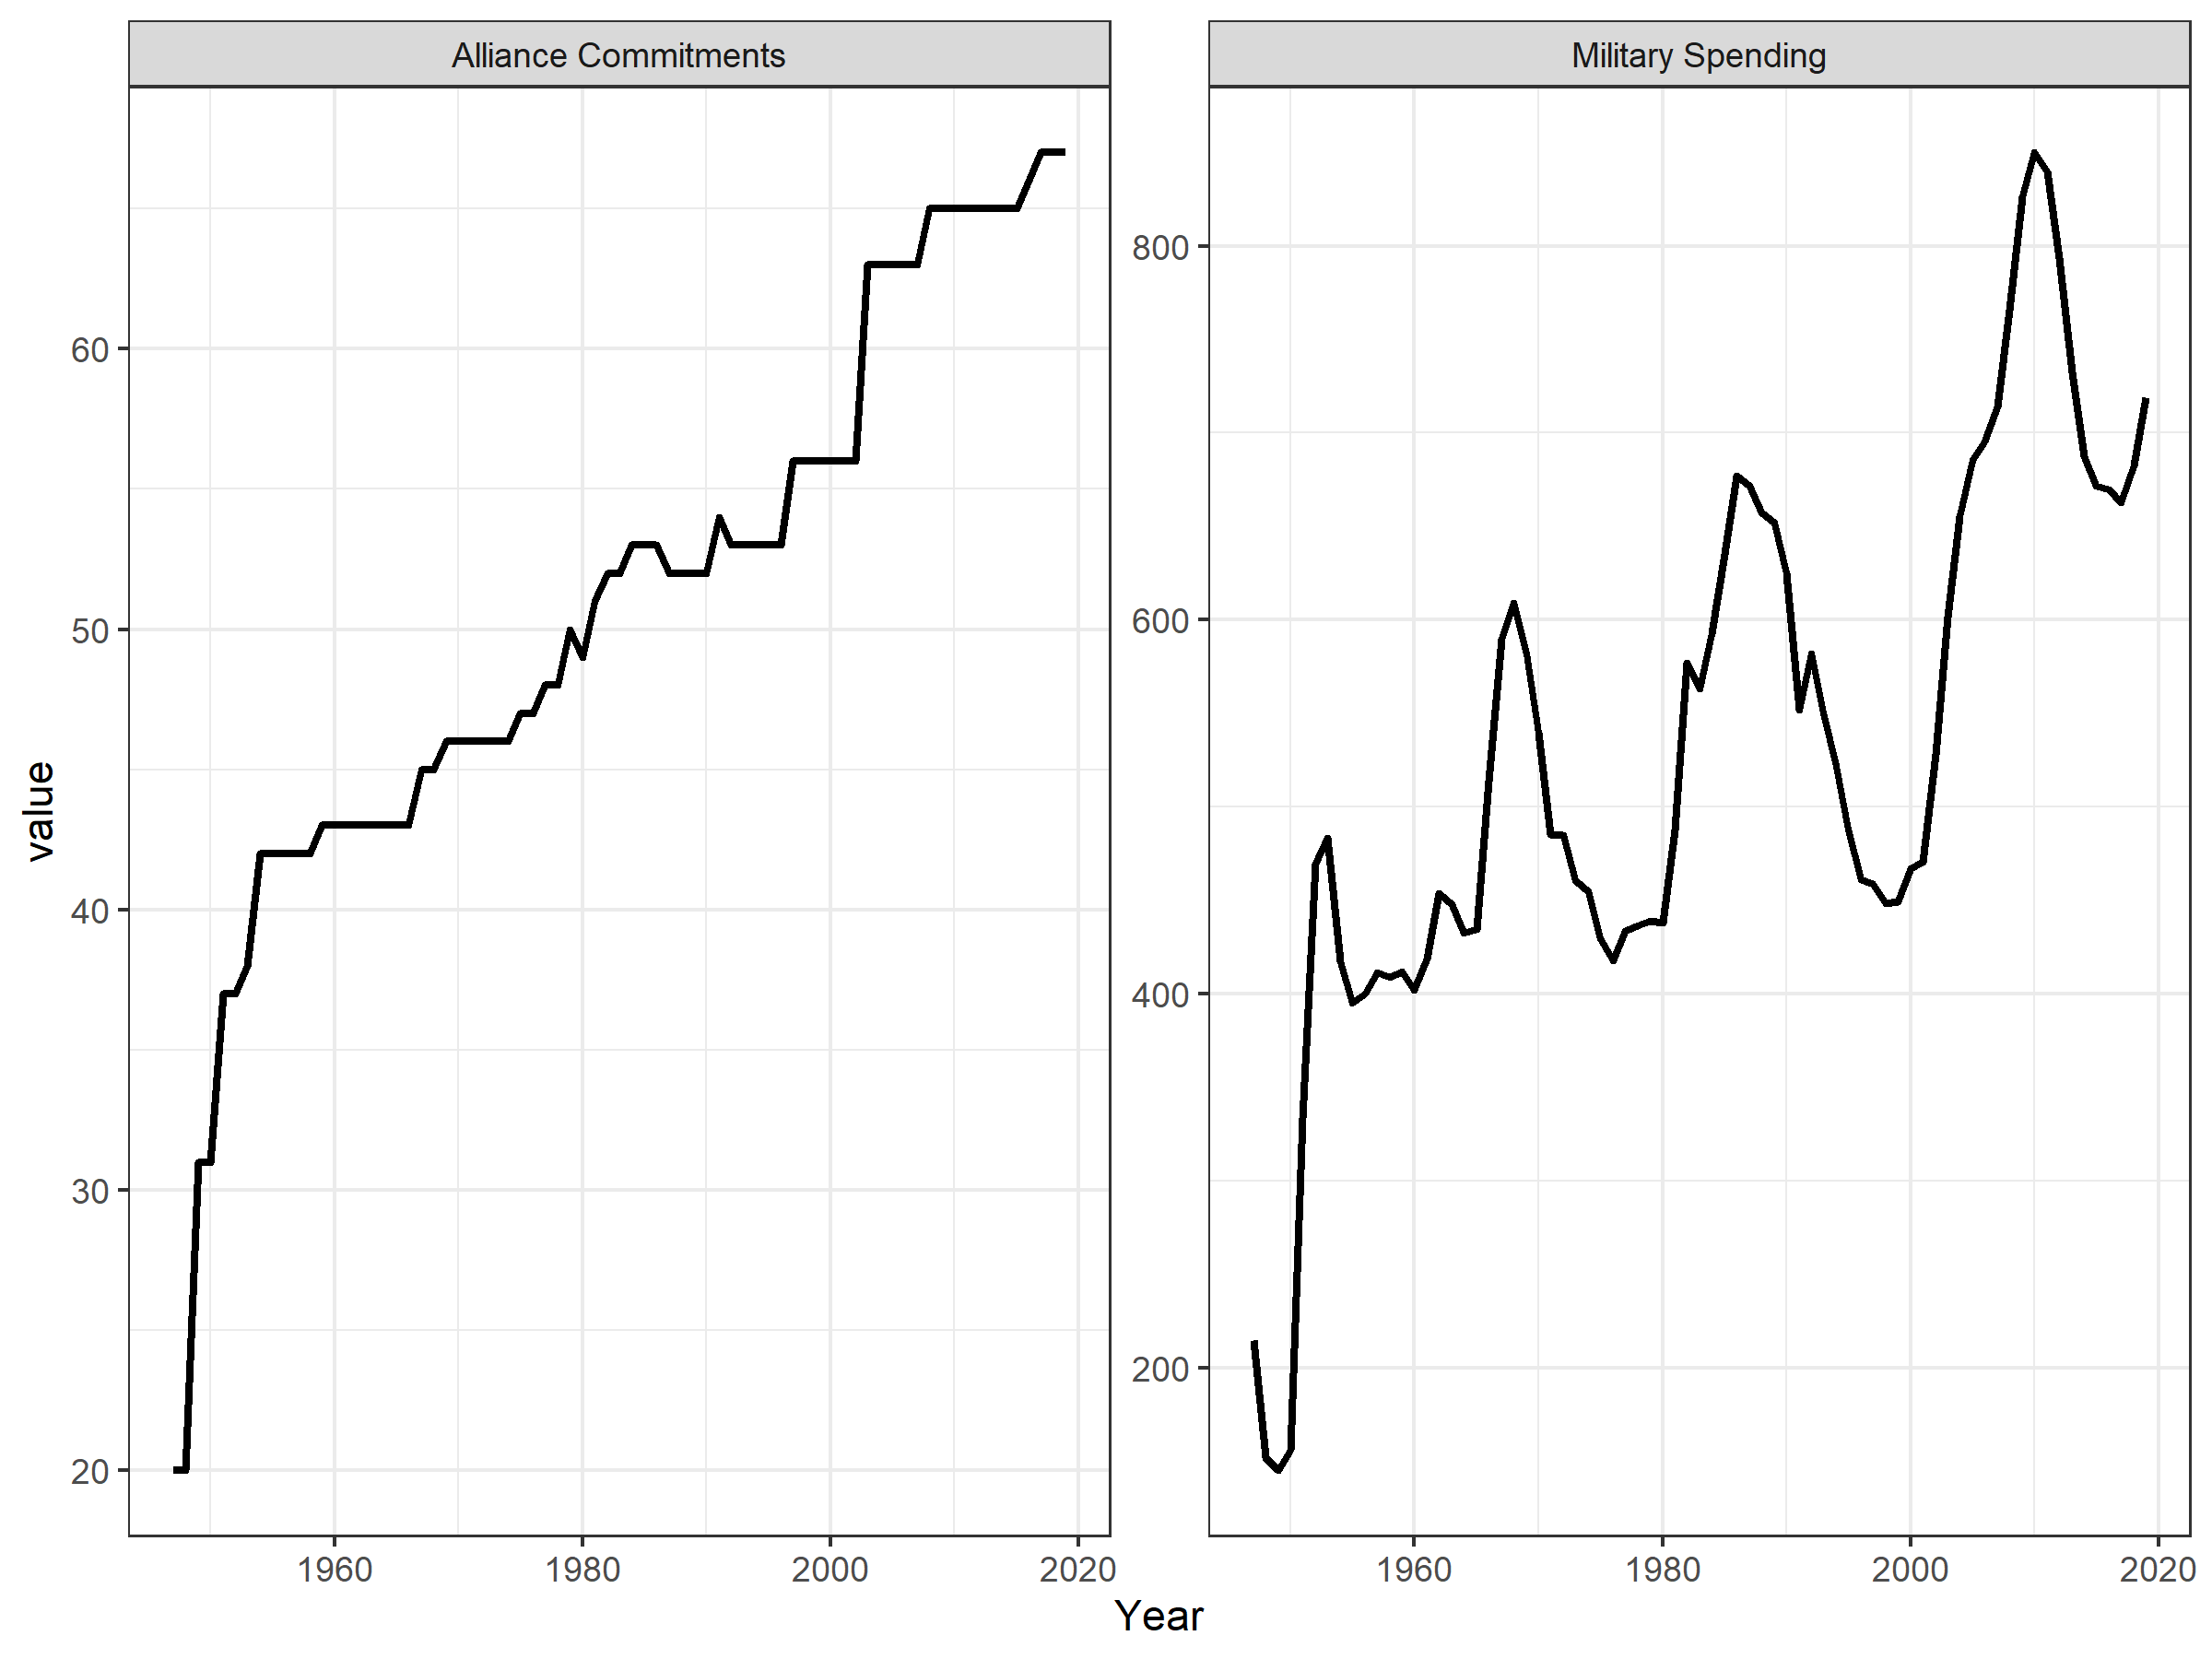
\includegraphics[width = .95\textwidth]{../figures/outcome-iv.png}
\caption{Time series of U.S. alliance commitments and defense spending from 1947 to 2019.}
\label{fig:outcome-iv}
\end{figure}


To accurately estimate the relationship between alliance commitments and military spending, we have to account for correlations between past and current values of both variables.
\autoref{fig:outcome-iv} suggests that both alliances and military spending are highly autocorrelated, meaning that past values of each variable seem to strongly predict current values. 
It is therefore possible that a simple correlation between these two variables could reflect simultaneous increases over time rather than a real relationship. 
Put differently, a standard regression with two autocorrelated or non-stationary variables could easily generate spurious findings.\autocite{GrangerNewbold1974}


% describe core of our model
Given persistence in alliance commitments and military spending over time, we use an autoregressive distributed lag model to estimate the correlation between alliances and defense spending.
The key independent variable in this model is the lagged number of alliance commitments, and we also use a one-year lag of military spending to predict current military spending. 
This regression model specification assumes that any effect of changing the number of U.S. alliances on military spending takes place over many years.
As the above discussion of the budget hawk and bargain hunter schools underscores, the financial burdens and savings generated by alliances may not necessarily happen immediately.


% Discuss form and uncertainty in regression models
Dynamic regression models can take many forms. 
Some models are best when the independent or outcome variable has long memory, otherwise known as a unit root.\footnote{Specifically, error correction models assume that the outcome and key variable are unit roots. We do not present error correction models in the paper, but we find some evidence of cointegration and very similar long-run effects of alliances with this specification.} 
The problem is that reliably identifying the dynamic properties of alliances, military spending, and other determinants of military spending is difficult. 
Existing tests for unit roots struggle to identify the specific dynamic properties of a series, especially in smaller samples or cases of high autocorrelation that are close to but less than integrated. 
Unit root tests for integration have low power and are very sensitive to specification choices like trend, drift, and lag length.\autocite{Webbetal2019}


% LRM test  
To overcome this issue, we use a more general and robust technique to identify whether there is a long-run relationship between alliances and military spending. 
A long-run relationship implies that changes in alliances dynamically affect military spending. 
To determine whether alliances and defense spending are in a long-run relationship, we employ a long-run multiplier bounds test.\autocite{Webbetal2020} 
This analysis uses coefficients from regression models to identify long-run relationships regardless of the dynamic properties of the outcome and independent variable and accommodates uncertainty about the dynamic properties of the variables. 
In our model, the bounds test uses the lagged alliance commitments and lagged military spending coefficient estimates. 
We find that the long-run multiplier estimate has a test-statistic greater than the upper bound of the long-run multiplier test.\footnote{To be precise, the long-run multiplier test statistic is 6.7 and the conservative upper bound is 3.59.} 
As a result, we can conclude that there is a long-run relationship between alliances and military spending.\autocite[293]{Webbetal2019} 


%MF: Given that we're calling attention to our small sample (which we should do), I wonder if we can add a footnote to reassure readers that this is still enough observations to draw meaningful inferences. I can see a non-quant person, in particular, thinking that this really undermines the case for our statistical approach. Maybe we could add a footnote pointing to other studies that have used a similar method with a similar sample size?
% JA: added the footnote. Let's keep this in mind as we revise, however. 
The testing procedure for long-run relationships performs well in small samples,\autocite{Webbetal2019} which is essential because we have 73 observations.
Such limited sample sizes are common in social science time series, and time-series methods in political science can make reasonable inferences with even smaller samples than ours.\autocite[See, for example,][]{OwenQuinn2014}
The small sample does increase uncertainty in our estimates, however. 
Based on these test results, we have sufficient confidence to proceed with using a dynamic regression technique to estimate the relationship between U.S. alliances and military spending. 
%\footnote{\cite{VolschoKelly2012} and \cite{OwenQuinn2014} are two examples of studies that estimate dynamic models with less than 60 observations.}



% introduce log model
In estimating the effect of alliance commitments on U.S. military spending, we consider two functional forms for the relationship. 
It is possible that as total U.S. alliances increase, the marginal cost of new alliances falls.
Perhaps adding one alliance when there are 40 alliance commitments is less costly than adding one alliance to 15 commitments, for example. 
Models with the total number of commitments assume that the effect of adding one alliance is roughly constant. 
In a second model, we relax that assumption by logging the number of alliance commitments before including the logged commitments variable in lags in the model. 
This transformation of the alliance commitments variable is a simple way to capture a potential non-linear relationship between alliances and U.S. military spending. 
The long-run multiplier bounds test suggests that there is also a long-run relationship between logged alliance commitments and military spending. 
One drawback of this approach, however, is that the log alliance commitments coefficient estimates have a less intuitive interpretation. 

% describe controls
Another concern is that an apparent relationship between alliance commitments and military spending could be driven by other factors. 
Changes in the international threat environment, for instance, could explain some of the contemporaneous movement in alliance formation and defense expenditures shown in Figure \ref{fig:outcome-iv}.
We control for several potential confounding variables to reduce omitted variable bias, which occurs when a statistical model does not account for factors that are correlated with the key independent variable and the outcome.\footnote{We consider additional control variables and many model specifications in the appendix, and show that our lagged alliance commitments coefficient is fairly consistent across model specifications.} 
We lag most of the control variables because we expect that, like alliances, changes in these factors affect the budget in the long-run. 

\begin{itemize}

\item \textbf{Log Combat Fatalities}. We included the log of annual U.S. military combat fatalities as a measure of international conflict intensity.\footnote{To get full coverage from 1947 to 2019, we compiled data on fatalities from three sources: \cite{mintzpolitical92}; the Defense Manpower Data Center; and icasualties.org.} More intense military threats increase defense expenditures and might also drive countries to seek more alliance partners. 

\item \textbf{Lag Major Power Rival Spending}. To account for the broader international threat environment, our model controls for lagged spending by all major power strategic rivals.\footnote{We identified strategic rivalry years with Russia and China using data from \cite{ThompsonDreyer2012}. We then combined rebased data from the Correlates of War and SIPRI to measure Russian and Chinese military spending. See the appendix for results with a variety of other threat controls, including interstate disputes, international crises, and just Russian spending.}

\item \textbf{Post-Conflict Years}. We included a dummy indicator for the five years after a war ends to capture post-conflict peace dividends and the reduced need for alliances once hostilities end.  

\item \textbf{Cold War}. To account for the superpower competition between the United States and the Soviet Union, which drove up spending and alliance formation, we control for Cold War years with a binary indicator.\footnote{The Cold War dummy variable is equal to one before 1991 and is zero afterwards.}



\item \textbf{Lag Change in GDP}. We control for economic growth because the United States had more resources to invest in defense and military alliances during periods of economic prosperity.

\item \textbf{Lag Budget Deficit}. As a second indicator of the opportunity costs of military spending, we account for the lagged budget deficit. 

\item \textbf{Republican President}. We control for presidential partisanship with a lagged dummy indicator for whether the president was a Republican, as Republican leaders tend to be more hawkish and wary of international entanglements.

\end{itemize}
  
Additional presidential administration-specific factors could also influence alliances and defense spending. Although U.S. grand strategy has been relatively constant since 1945, there have been differences in national security priorities across presidents. As described below, after presenting our initial results, we account for these differences by adding presidential fixed effects to our models. 

%On the security front, we included the log of annual U.S. military combat fatalities as a measure of international conflict intensity.\footnote{To get full coverage from 1947 to 2019, we compiled data on fatalities from three sources: \autocite{mintzpolitical92}; the Defense Manpower Data Center; and icasualties.org.}
%We also included a dummy indicator for the five years after a war ends to capture post-conflict peace dividends and the reduced need for alliances once hostilities end.  
%To account for the superpower competition between the United States and the Soviet Union, which drove up spending and alliance formation, we control for Cold War years and Soviet/Russian military spending.\footnote{The Cold War dummy variable is equal to one before 1991 and is zero afterwards. We used a combination of data from the Correlates of War and SIPRI to construct the Russian spending measure.}
%We also controlled for economic factors, as these might shape the opportunity costs of military spending\autocite{Zielinskietal2017,norrlofCMPS19} and change how policymakers assess the burdens of international commitments.  
%Our main economic controls are lagged changes in GDP and lagged budget deficit.
%Finally, we controlled for presidential partisanship with a lagged dummy indicator for whether the president was a Republican, as Republican leaders tend to be more hawkish and wary of international entanglements.\footnote{We also consider other control variables and many model specifications in the appendix, and show that our lagged alliance commitments coefficient is fairly consistent across model specifications.} 




\section*{Findings}


\autoref{tab:adl-coefs} provides the results from our regression models of U.S. defense expenditures from 1947 to 2019. 
Model 1 uses the total number of security guarantees to construct our independent variables and Model 2 is based on logged alliance commitments. 
%The first thing to note is that past levels of military spending help predict current spending, which is unsurprising. 


\begin{table}[!htbp] \centering 
\begin{tabular}{@{\extracolsep{5pt}}lcc} 
\\[-1.8ex]\hline \\[-1.8ex] 
\\[-1.8ex] & \multicolumn{2}{c}{Military Spending} \\ 
\\[-1.8ex] & (1) & (2)\\ 
\hline \\[-1.8ex] 
 Lagged Military Spending & 0.387$^{}$ & 0.440$^{}$ \\ 
  & (0.251, 0.524) & (0.300, 0.581) \\ 
  Lag Alliance Commitments & 9.670$^{}$ &  \\ 
  & (6.796, 12.544) &  \\ 
  Lag Log Alliance Commitments &  & 273.668$^{}$ \\ 
  &  & (180.698, 366.639) \\ 
  Lag Change in GDP & $-$0.060$^{}$ & $-$0.024 \\ 
  & ($-$0.128, 0.008) & ($-$0.094, 0.045) \\ 
  Lag Major Rival Spending & 0.027 & 0.076 \\ 
  & ($-$0.075, 0.129) & ($-$0.025, 0.176) \\ 
  Cold War & 25.708 & $-$33.299 \\ 
  & ($-$49.418, 100.834) & ($-$101.715, 35.116) \\ 
  Post-Conflict Years & $-$9.381 & $-$13.377 \\ 
  & ($-$36.015, 17.252) & ($-$41.204, 14.450) \\ 
  Log Combat Fatalities & 8.938$^{}$ & 9.384$^{}$ \\ 
  & (5.018, 12.857) & (5.269, 13.499) \\ 
  Lag Republican President & 19.215 & 22.925$^{}$ \\ 
  & ($-$4.582, 43.013) & ($-$1.932, 47.781) \\ 
  Lag Budget Deficit & $-$0.418 & $-$1.651 \\ 
  & ($-$7.266, 6.429) & ($-$8.842, 5.539) \\ 
  Constant & $-$202.501$^{}$ & $-$802.537$^{}$ \\ 
  & ($-$351.566, $-$53.435) & ($-$1,165.185, $-$439.888) \\ 
 N & 73 & 73 \\ 
\hline \\[-1.8ex] 
\multicolumn{3}{l}{95\% Confidence Intervals in Parentheses.} \\ 
\end{tabular} 
\caption{Coefficient Estimates from an autoregressive distributed lag regression model of U.S. alliance commitments and military spending from 1947 to 2019.
                  %The dependent variable is annual military spending, measured in billions of 2011 U.S. dollars.
                  %The key independent variable is a one year lag of U.S. alliance commitments in each year, either without any transformation or in logs.
                   } 
\label{tab:adl-coefs}
\end{table}


The coefficient on the alliance commitments variable is positive and the 95 percent confidence intervals exclude zero in Models 1 and 2. 
This suggests that alliance commitments are positively correlated with defense expenditures, as the budget hawk school expects, regardless of whether we model this relationship as linear (Model 1) or characterized by diminishing marginal costs (Model 2). 
Although the direction of the effect is informative, statistical significance is a poor indicator of substantive importance.\autocite{McCaskeyRainey2015}
We want to know the magnitude of the association between alliance commitments and U.S. spending, not just whether the p-values are below a certain threshold. 

The alliance commitments coefficient captures the effect of adding one new security guarantee on the next year's defense budget.
Based on Model 1, adding one additional commitment increases U.S. defense spending the next year by \$9.8 billion.
The 95 percent confidence interval indicates that the short-run effect could range between \$6.8 and \$12.5 billion.
Independent variables have a less intuitive interpretation when they are log-transformed, but Model 2 similarly yields a potentially large substantive effect. 
A 10 percent increase in the logged changes in alliance commitments leads to about \$29 billion more in defense spending the next year, with a 95 percent confidence interval ranging from \$22.3 billion to \$35.6 billion.

Much of the cost (or savings) associated with alliances might not materialize just one year later. 
Because changes in military spending accumulate over time, the impact of a new alliance commitment is spread out over multiple years. 
The United States and Taiwan forged a formal defense pact in 1954, for instance, but U.S. troop levels on the island did not peak until four years later.\autocite{kaneglobal04} 
The long-run costs of an alliance, then, give a more complete sense of their financial toll than the regression coefficients alone. 
We use the long-run multiplier of alliance commitments to capture the \textit{total} effect of a one unit increase in the lagged number of alliance commitments on defense spending. 
To calculate the long-run multiplier, we divide the lagged alliance commitments coefficient by the lagged level of military spending coefficient and calculate standard errors with the delta method.\footnote{Formally, this is equal to $\frac{\mbox{Lagged Alliance Commitments Coefficient}}{(1 - \mbox{Lagged Spending Levels Coefficient})}$. This long-run multiplier is the basis of the long-run multiplier test we used to assess the presence of a long-run relationship.} 

The long-run multiplier of a new alliance commitment is positive and large: one additional alliance commitment ultimately adds between \$11 and \$21 billion to the defense budget, on average, according to Model 1.
Put differently, the annual level of the defense budget is \$11 to \$21 billion greater once the impact of making a new alliance commitment is fully realized.
This estimated range is a 95\% confidence interval based on a point estimate of 15.8 and a standard error of 2.6. 
Based on the estimates from Model 2, a 10 percent increase in logged alliance commitments adds \$51 billion in spending over the long-run, with a 95 percent confidence interval that spans from \$36 billion to \$68 billion.


To further illustrate our results, we assess the substantive impact of a well-known change in U.S. alliance commitments: NATO expansion after the Cold War. 
This part of the analysis answers recent calls for further scrutiny of NATO expansion, which was an extremely consequential policy decision.\autocite{GoldgeierShifrinson2020}
We focus on the admission of the three Baltic States in 2003-04. 
Offering NATO membership to Estonia, Latvia, and Lithuania was unique and controversial because they were formerly part of the Soviet Union.
What was the budgetary impact of making formal defense commitments to three former Soviet states?  


To find out, we carried out a counterfactual analysis. 
First, we simulated a set of coefficient estimates using the results from the regression model.\footnote{The simulation uses the central limit theorem to simulate a distribution of coefficients from the model estimates, then multiplies the simulated parameter vectors by two datasets -- one with the observed data and the other with hypothetical data.}
We then used the model estimates to make predictions in two scenarios: one with the observed NATO expansion into the Baltic States and the other in a hypothetical scenario where NATO did not expand. 
In the latter analysis, we remove the three Baltic alliance commitments and hold all other factors constant except the lagged level of spending.
This means that the counterfactual data contains three fewer U.S. alliance commitments relative to the observed number of alliances after 2004. 
The counterfactual analysis predicts spending in each year, then uses the predicted values as the lagged spending value in the next period, which allows us to fully express the impact of the hypothetical change in alliances.\footnote{Because annual predictions in the counterfactual are based on simulated lagged spending values after 2004, there is more uncertainty in the counterfactual estimates than the observed data, which draw on a single lagged spending value instead of multiple simulated values.}
The difference in spending between these two scenarios provides an estimate for the budgetary cost of NATO expansion.


%MF: edits here for clarity, moved up some text from below to summarize main point.
\autoref{fig:nato-counterfactual-adl-nolog} plots the results. 
The bottom panel shows 95\% confidence intervals for predicted changes in U.S. military spending, with the observed case depicted in black and the hypothetical non-expansion scenario shown in gray.
The top panel shows the 95\% confidence interval for the difference between the predictions with the observed data and predictions with the counterfactual data. 
The figure makes clear that NATO expansion into the Baltic states consistently led to higher military spending. 
By 2019, the estimated difference between the observed and counterfactual scenarios is between \$13 and \$46 billion. 
These costs reflect substantial investments in infrastructure and increased NATO membership expenses.\autocite{Moller2020}
Further expenditures support allied training, procurement and more recently, the European Deterrence Initiative.\autocite{CRS2020} 
NATO expansion is also associated with a perceptible difference in U.S. military spending when we log-transform the alliance commitments variable, but the estimated effects are more uncertain. 
As shown in the online appendix, the estimated difference between adding the Baltic states and keeping them out of NATO is between \$1 and \$40 billion by 2019, all else equal. 

\begin{figure} 
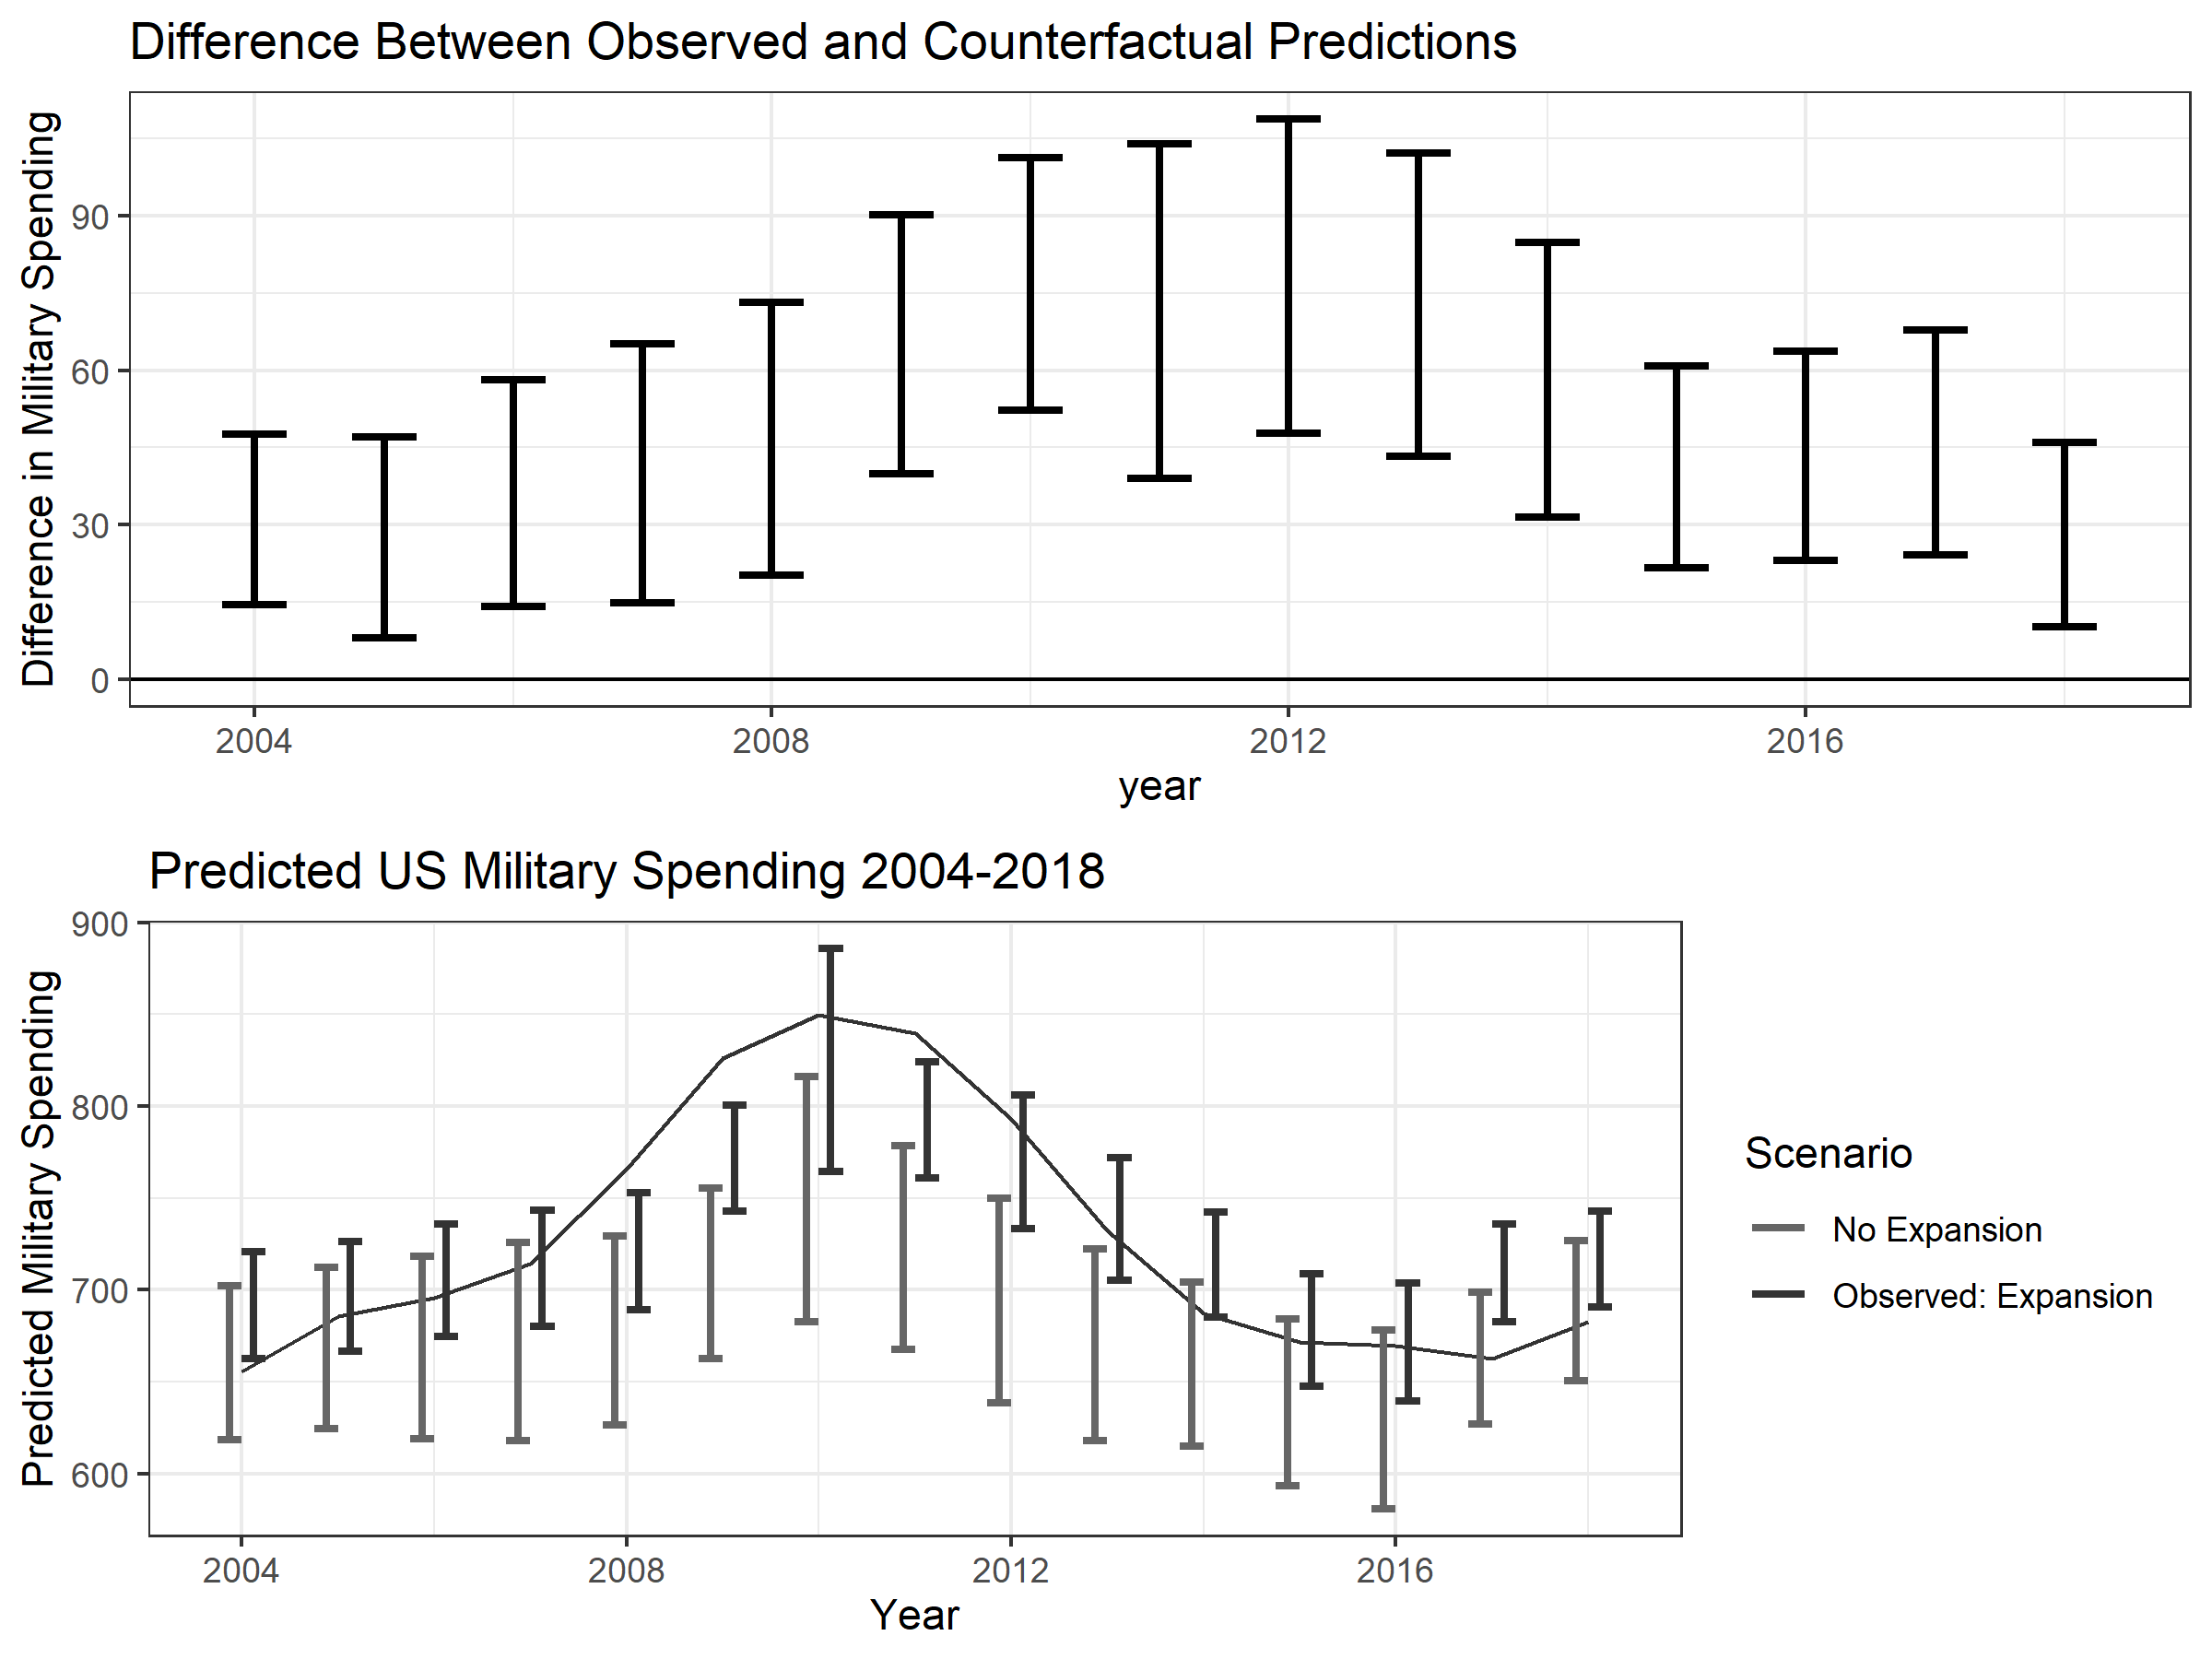
\includegraphics[width = .95\textwidth]{../figures/nato-counterfactual-adl-nolog.png}
\caption{Estimated U.S. military spending with and without NATO expansion to Estonia, Latvia and Lithuania. 
The bottom panel shows predictions from two circumstances: (1) observed NATO expansion and (2) a counterfactual scenario where NATO did not add the three Baltic countries in 2004. 
The top panel plots the estimated annual difference between predictions from the observed data. 
The error bars summarize the 95\% confidence interval for the predicted values and differences.
Estimates on the scale of billions of dollars.}
\label{fig:nato-counterfactual-adl-nolog}
\end{figure}


% cut the logged commitments figure
\begin{comment}
To make substantive predictions about the impact of logged alliance commitments, we repeated the NATO counterfactual simulation. 
\autoref{fig:nato-counterfactual-adl-log} plots these results, which are based on the estimates in the second column of \autoref{tab:adl-coefs}. 



\begin{figure} 
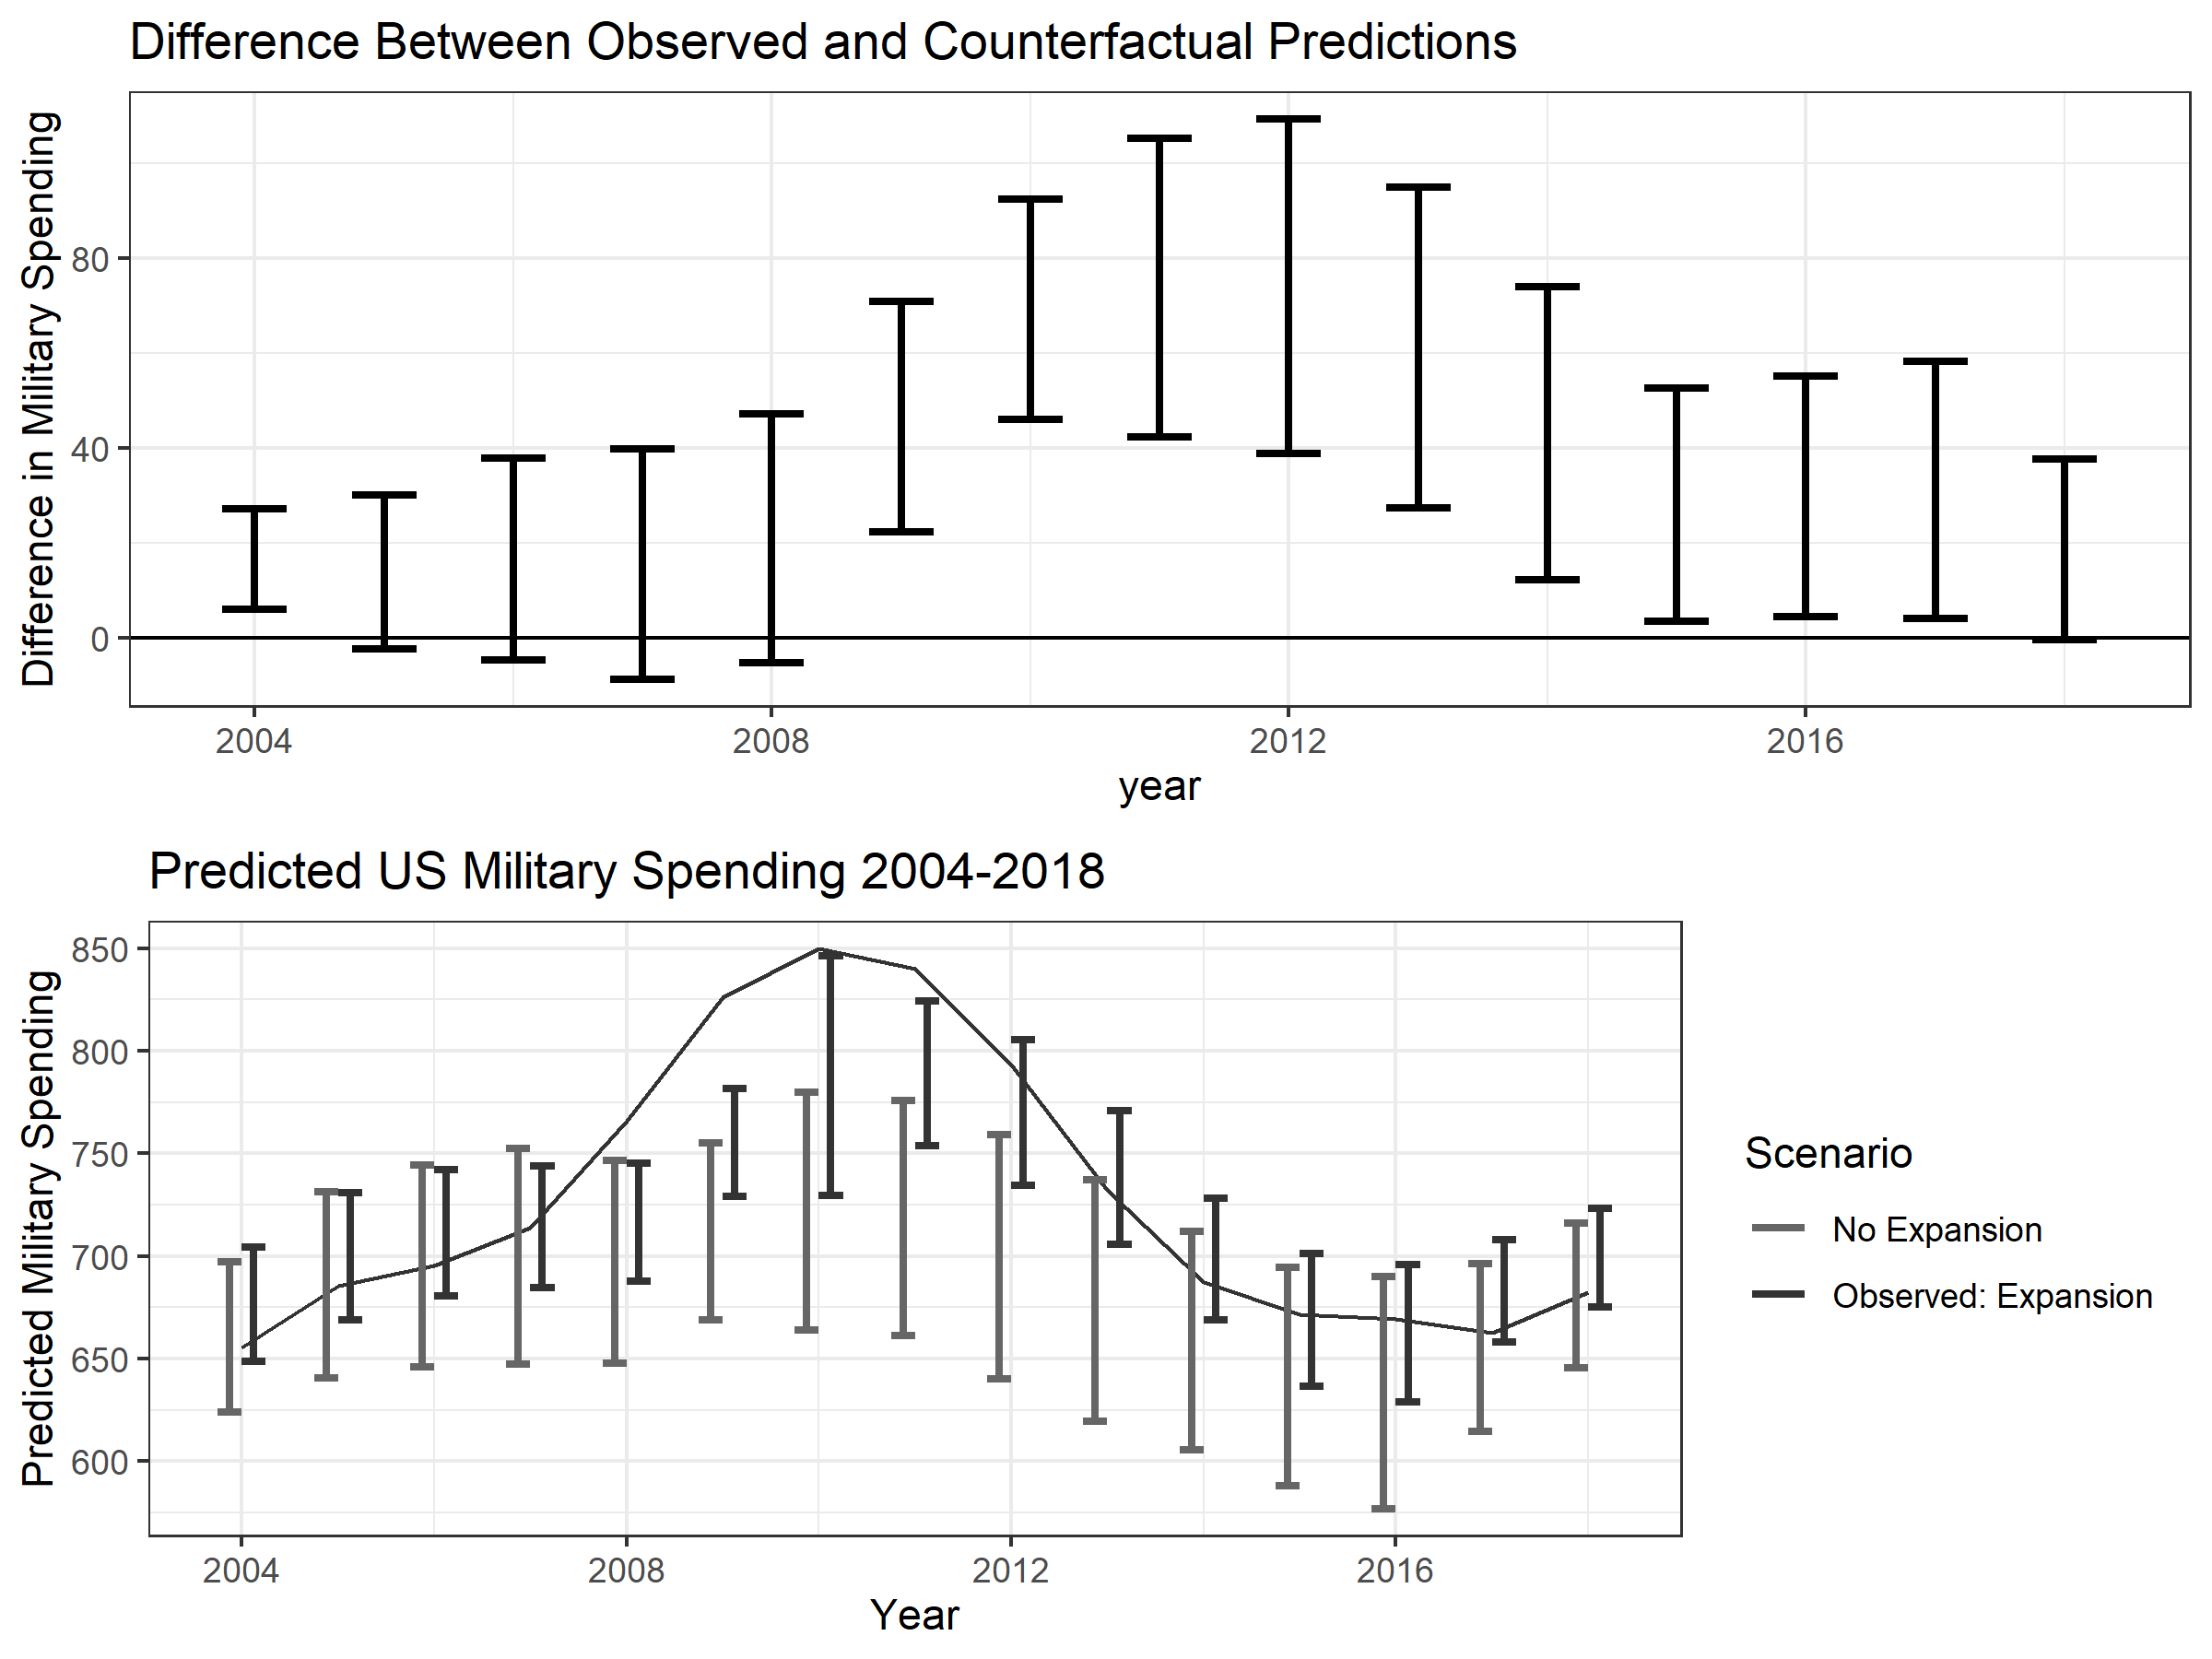
\includegraphics[width = .95\textwidth]{../figures/nato-counterfactual-adl-log.png}
\caption{Estimated U.S. military spending with and without NATO expansion to Estonia, Latvia and Lithuania. 
This simulation uses logged alliance commitments as the key independent variable. 
The bottom panel shows predictions from two circumstances, first the historic NATO expansion from 2004, and the other from counterfactual data where NATO did not add these three members. 
The top panel plots the estimated annual difference between predictions from the observed data. 
The error bars summarize the 95\% confidence interval for the predicted values and differences.
Estimates on the scale of billions of dollars.}
\label{fig:nato-counterfactual-adl-log}
\end{figure}


NATO expansion is associated with a perceptible difference in U.S. military spending, even after log-transforming the alliance commitments variable, though the estimated effects are smaller. 
By 2019, the estimated difference between adding the Baltic states and not is between \$5 and \$41 billion, all else equal. 
Therefore, logging alliance commitments leads to very similar inferences about the relationship between alliances and U.S. military spending. 

\end{comment}
  
% sum up the findings
%MF: edits here
In sum, we find that taking on more alliance commitments is associated with increased military spending, all else equal.
Adding a single alliance commitment to the U.S. portfolio adds billions of dollars to the defense budget, on average, in the long run.
These conclusions do not depend on assumptions about the marginal cost of alliances, as inferences with logged alliance commitments are very similar. 
These results are consistent with the budget hawk view that alliance participation increases U.S. military spending, and contradict the bargain hunter perspective.
However, before reaching more definitive conclusions, it is important to assess the robustness of our findings. 
We take up this task in the next section. 



\subsection*{Robustness Checks}

Our findings could be driven by unusual and influential observations, especially since our sample is relatively small. 
U.S. military spending and alliances both increase dramatically between 1949 and 1951, as the Korean War drove large spending increases and the United States formed some key Cold War alliances.
There is another sharp increase in both defense expenditures and alliance commitments shortly after the 9/11 attacks.  
We assess whether these periods or other transient shifts in the international context drive our results in three ways.


First, we estimate models in a different samples, including one that starts in 1954 instead of of 1947 and another that starts in 1920.\footnote{The latter results, which include a pre-World War II period when the United States did not provide any security guarantees, appear in the online appendix.}
Starting in 1954 eliminates any impact of data from the unusual immediate postwar period on our estimates. 
Second, we add two dummy variables -- one for all years before 1953 and another for the period after 9/11 -- to control for these unique periods. 
Third, we include presidential fixed effects in our model.
Administration-specific binary variables control for unobserved confounding factors that may be specific to presidential administrations.
This accounts for unusual administration-specific changes, such as the Reagan defense buildup and the global war on terror, as well as changes in U.S. foreign policy priorities.\footnote{In the models with president-specific binary variables, we drop the Cold War and Republican president control variables, as these indicators are perfectly correlated with some presidential fixed effects.} 


\begin{figure} 
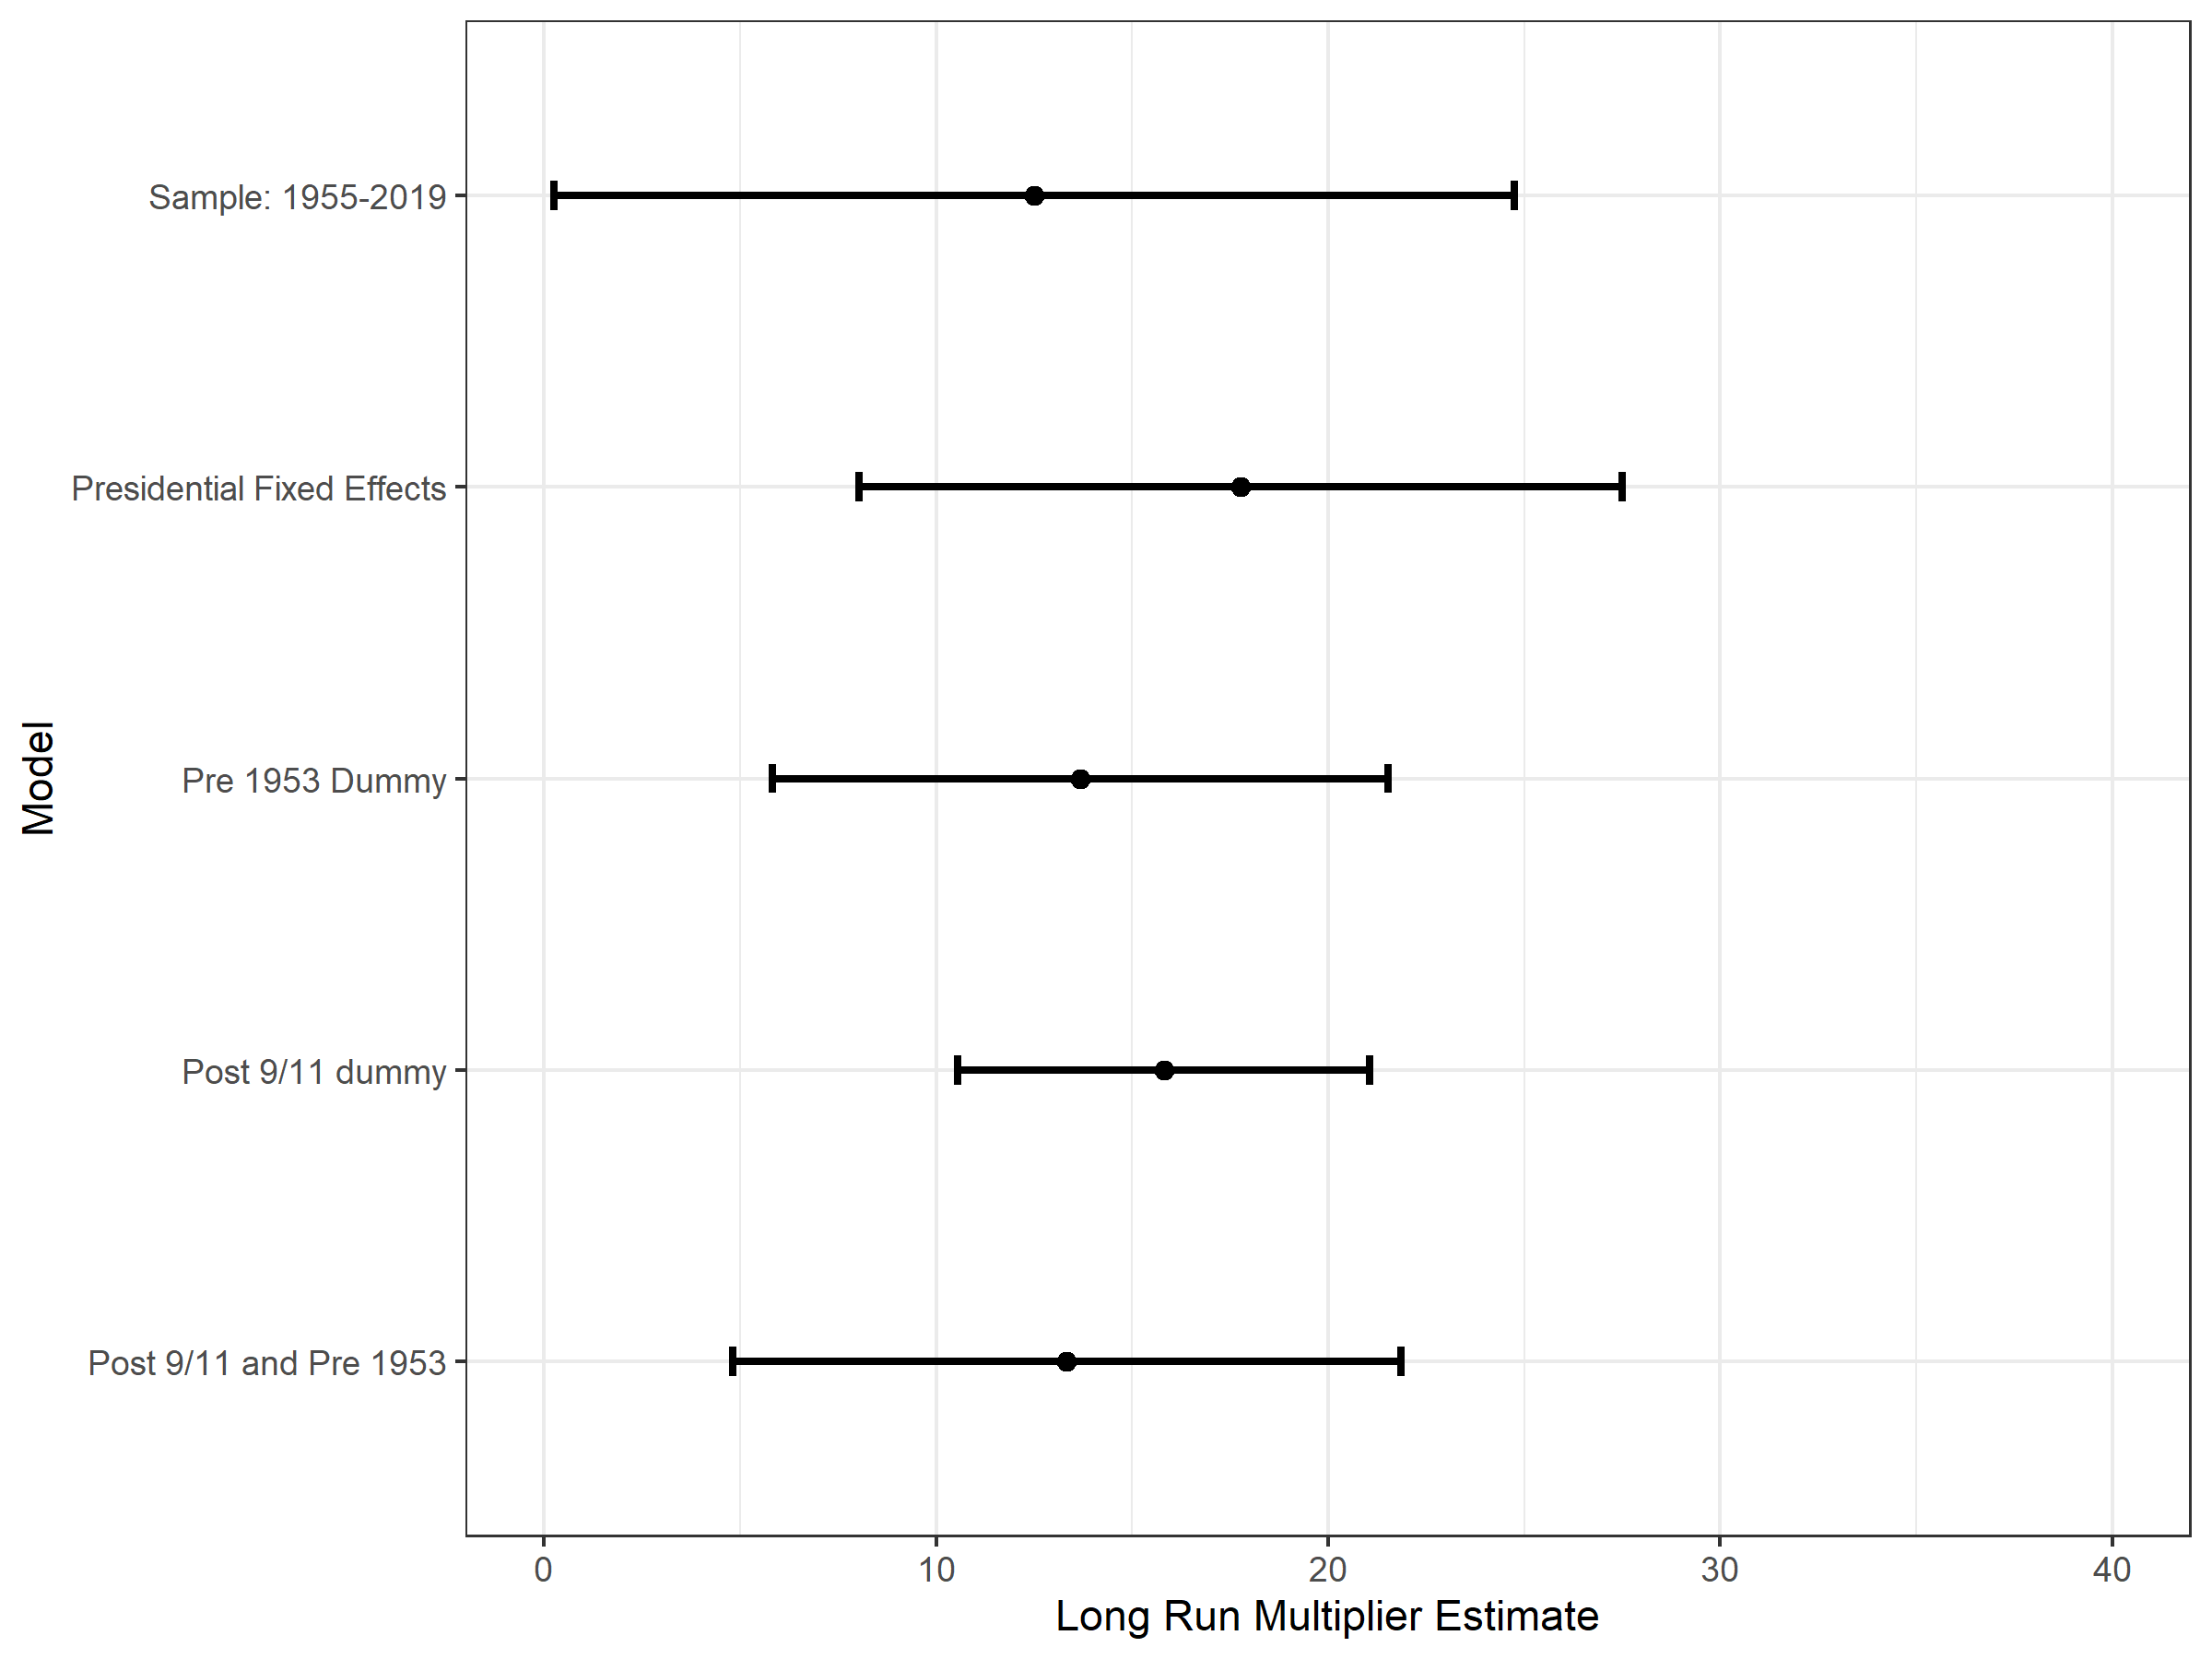
\includegraphics[width = .95\textwidth]{../figures/lrm-rob.png}
\caption{Estimated long-run multiplier of a one-unit increase in U.S. alliance commitments across different samples and model specifications. 
The y-axis contains information about how the model or sample deviates from our baseline regression model. 
Points mark the expected value, while the error bars summarize the 95\% confidence interval.
Estimates on the scale of billions of dollars. }
\label{fig:lrm-rob}
\end{figure}


%MF: light editing and further drawing out of implications from the FE model. 
\autoref{fig:lrm-rob} summarizes how these changes alter our initial results. 
The figure reports the estimated long-run multipliers of a one-unit increase in U.S. alliance commitments for each model.
These estimates suggest that our substantive conclusions about the relationship between alliances and military spending are relatively unaffected by unusual periods of alliances and defense spending after World War II.
There are slight differences in the estimates across the different specifications, largely because of our small sample size, but the substantive inferences are broadly similar. 
Most models find a more uncertain long-run effect than our original model (\$11 to \$21 billion), but there is little appreciable difference in the estimates.  
The biggest estimated effect emerges from the model that adds presidential fixed effects to our baseline specification.
This model suggests that the long-run impact of adding an alliance is about \$18 billion, compared to \$16 billion in our main analysis. 
Adding presidential fixed effects increases uncertainty in the long-run multiplier, as this model has twelve fewer degrees of freedom. 
%That we continue to find large positive increases in the fixed effects model means that within the same administration taking on new commitments increases defense spending. 
Our results cannot be explained, therefore, by changes in foreign policy or grand strategy among different presidents.



We present the results from further robustness checks in an online appendix. 
First, we conduct an extreme bounds analysis that involves re-running our model 12,911 times with different combinations of independent variables.
This analysis allows us to determine whether our results are sensitive to the model specification we chose.
Second, we estimate error correction models as an alternative way to specify dynamic regression models.
Third, we estimate static models with alliances and military spending in first differences.
Fourth, we use an alternative lag structure in the ADL model, and find a slightly smaller substantive effect of \$6 to 15 billion per alliance when we include two lags of defense spending. 
Last, we analyze data from 1920 on to capture the impact of alliances starting with no commitments. 
All of these checks come to the same substantive conclusion: alliance participation is associated with greater U.S. military spending.
%The evidence consistently favors the budget hawk view of alliances. 

%As another way to account for the influence of unusual observations, we replicate our analysis using robust regression estimators. 
%This allows us to analyze two additional periods of time: 1945-2019 and 1949-2019 (recall that our main models start in 1947). 


%``Moreover, even under the rosiest scenarios, curtailing America’s alliance military com- mitments would save something in the vicin- ity of 1 percent of gdp''
%https://www.jstor.org/stable/26557320?casa_token=ej5vXAXtQx4AAAAA%3Ak3OHJPMegfFA6ZFOZwEVMasbLm_RSDLUU5dukz1LNhLRmyUOZKOMhA0GUyEk783AZtYmsdRQWFbuK3J85j9Qqua6xsWSl3LE0bWzZQv9cqTV5N4Bcw&seq=1#metadata_info_tab_contents

%If the United States could achieve its military policy goals, other than pro-moting global stability, with a $150 billion defense budget—that is, if the United States only requires the rest of the force to maintain the alliances and sustain the operations that enhance stability—then the budgetary cost of the stability mission is $150 billion.
%https://www.tandfonline.com/doi/pdf/10.1080/09636410108429444?casa_token=sfy6T7MDJrAAAAAA:d0hHmbbUY7Gol5zZJq55E9kwPVkcPPLC3UYtI1jzeNxDDIrrRsXjtwitRDGXGNqCcW88tWsfUoE , p. 54
 
%Posen: ``I have argued that if the United States were more judicious in its promises abroad, perhaps a fifth of the defense budget could be cut (excluding the costs of actual wars), amounting to roughly one hundred billion dollars per year at current prices. ''

%Some figures on the costs of overseas troop deployments: https://theconversation.com/why-does-the-us-pay-so-much-for-the-defense-of-its-allies-5-questions-answered-127683

%From Beckley: ``14. Eugene Gholz, Daryl G. Press, and Harvey M. Sapolsky, “Come Home, America: The Strategy of Restraint in the Face of Temptation,” International Security, Vol. 21, No. 4 (Spring 1997), pp. 5–48; Layne, The Peace of Illusions, chap. 8; Ted Galen Carpenter, Smart Power: Toward a Prudent Foreign Policy for America (Washington, D.C.: CATO Institute, 2008); and Benjamin H. Friedman, Brendan Rittenhouse Green, and Justin Logan, “Correspondence: Debating American Engagement—The Future of U.S. Grand Strategy,” International Security, Vol. 38, No. 2 (Fall 2013), pp. 183–192.''


\section*{Discussion and Conclusion}
 
Military alliances figure prominently in debates about U.S. grand strategy and foreign policy. This article investigated the financial cost of U.S. alliance commitments. We summarized two schools of thought that offer contradictory answers: the budget hawk school and the bargain hunter perspective. The former suggests that alliances generate large increases in defense expenditures, while the latter claims that security guarantees are relatively cheap and may even save the United States money in the long run. To assess these competing predictions, we designed a statistical model to estimate how changes in the number of alliance commitments over time affect U.S. defense expenditures while controlling for confounding factors, such as the president's political party and economic growth. Our approach accounts for the financial costs and benefits of U.S. security guarantees, including things that are difficult to measure directly, such as savings from extended deterrence and spending to compensate for ``free-riding'' by allies. 

We found that increasing the number of U.S. alliance commitments is associated with greater defense expenditures. In the long-run, on average, one additional alliance commitment adds between \$11 and \$21 billion to the level of the defense budget. Our models identify the general trend -- an important first step -- but cannot tell us the true budgetary burden of any single alliance. Some alliance commitments may exceed the \$11 and \$21 billion range, while others are almost certainly below it. Our analysis showed, for example, that post-Cold War NATO expansion into the Baltic States added between \$16 and \$45 billion to the defense budget, an average of between \$5.33 and \$15 billion per country. Other U.S. alliances, such as the one with Haiti, are undoubtedly even cheaper. 

A series of follow-on analyses showed that changing our research design in various ways can increase or decrease the range of our initial estimate. In each case, however, the results reaffirmed that increases in alliance commitments are correlated with large long-run growth in the defense budget. The increase in defense spending resulting from an additional alliance commitment is smallest (\$6 to \$15 billion) when we include two lags of defense spending in our model rather than one. 

The United States obviously does not form alliances at random. It is therefore possible that the factors giving rise to security guarantees -- rather than the commitments per se -- account for our results. We addressed this by controlling for factors that affect defense spending and alliance formation and are possible to measure, like expenditures by major power rivals and presidential partisanship. To account for unobservable confounders that do not change over time within the same administration, we estimated models with presidential fixed effects. This further reduces the risk of omitted variable bias, but these results could still be off the mark if there are one or more unaccounted for factors that change over time within the same administration and also cause both alliance formation and military spending. Although we cannot be certain that our findings reflect a causal relationship, at the very least, there is a strong positive association between alliance commitments and U.S. defense expenditures.

The fixed effects analysis is helpful for evaluating a key claim made by some scholars in the bargain hunter school: that U.S. defense spending on power projection capabilities and overseas deployments reflects grand strategy rather than alliance commitments specifically. Rapp-Hooper argues, for example, that ``America's spending reflects the country's far-flung global strategy, not its alliance commitments per se.''\autocite[100]{rapphoopershields20} If that were true, we would not expect to see differences in defense spending following changes in alliance commitments \textit{within the same administration}. That is because grand strategy, as well as beliefs about military spending and foreign policy more generally, are relatively stable within administrations. However, we find that the same presidential administration increases spending after extending security guarantees to additional countries. This suggests that alliances themselves -- not just U.S. grand strategy -- are responsible for at least some U.S. defense spending for overseas endeavors.  

%We also used presidential fixed effects to account for administration-specific confounders that do not change over time. Within the same administration, when the president's beliefs about military spending and foreign policy are relatively stable, we find that taking on an additional alliance commitment is associated with a large spending increase. Our fixed effects analysis further reduces the risk of omitted variable bias, but these results could still be off the mark if there are one or more unaccounted for factors that change over time within the same administration and also cause both alliance formation and military spending. Although we cannot be certain that our findings reflect a causal relationship, at the very least, there is a strong positive association between alliance commitments and U.S. defense expenditures.
%These results may not reflect a causal relationship. 
%Scholars have argued that U.S. defense spending on power projection capabilities and overseas deployments reflects grand strategy rather than alliance commitments specifically.  Rapp-Hooper argues, for example, that ``America's spending reflects the country's far-flung global strategy, not its alliance commitments per se.''\autocite[100]{rapphoopershields20} Overseas deployments 

Overall, our findings are consistent with the budget hawk claim that alliance commitments require the United States to shoulder a significant financial burden. They contradict the bargain hunter argument that the savings generated by alliances offset whatever expenses they require, leading to a net-neutral effect on the defense budget. Alliances may result in some efficiency gains, but their financial toll swamps any such savings for the United States. 

%Bargain hunters often argue that the savings generated by alliances offset whatever expenses they require, leading to a net-neutral effect on the defense budget.\footcite[See, for example,][]{rapphoopershields20,colbyTNI16} We have shown that this is not the case. Alliances may result in some efficiency gains, but their financial toll swamps any savings that the United States derives. 

The size of the budgetary burden stemming from alliances reflects -- and may exceed -- the expectations of the budget hawk school. Posen's estimate indicates that the United States could save about \$100 billion annually by being ``more judicious in its promises abroad.''\footcite{posenTNI16} Based on our analysis, U.S. alliance commitments may be responsible for a greater share of the defense budget than this estimate implies. We find that just one additional alliance commitment is associated with an annual increase to the defense budget between one-tenth and one-fifth of the \$100 billion estimate.
%Colby and Thomas, who are more sanguine about the costs of alliances, call this estimate the ``rosiest'' scenario, meaning that this is the most the United States could possibly save by paring back its alliance commitments.\footnote{\autocite[37]{colbyTNI16}. They write specifically that curtailing alliance commitments would save 1 percent of GDP. We assume this refers to Posen's claim, which serves as the basis for the \$100 billion estimate, that the United States could reduce defense expenditures from 3.5 to 2.5 percent of GDP.}
%MF: good point. But I think we need to compare our finding to what Posen concluded. I have revised the language here.
% JA: cut this- I'm not sure that's the right extrapolation from the model- we never see even -5 alliances in a year. 
%However, based on our analysis, U.S. alliance commitments may be responsible for a greater share of the defense budget than this estimate implies. Washington could get to \$100 billion in savings by eliminating between five and 10 alliance commitments. This translates to 7.5-15 percent of the security guarantees the United States is currently obligated to fulfill. 

%Making deeper cuts to the U.S. alliance portfolio could generate savings that goes well beyond \$100 billion annually. JA: This is the extrapolation problem- want to be careful here. 



Our findings stand in stark contrast to other research on military alliances and defense spending. Scholars usually assess this relationship by analyzing the behavior of a large number of countries over time. Many prior studies that take this approach conclude that alliances \textit{reduce} expenditures.\autocite[For a study that reaches a different conclusion, see][]{MorganPalmer2003} Matthew Digiuseppe and Paul Poast, for example, find that forming at least one alliance with a democracy decreases military expenditures by as much as 17.6 percent in the short-run, on average, compared to having zero alliances with democratic states.\autocite{DigiuseppePoast2016} Our analysis shows that the United States deviates from this general trend. Unlike other countries, the United States spends billions of dollars more on defense with each additional alliance commitment it makes. That other countries reduce their expenditures after forming alliances may be partially why the United States needs to increase its own. 

With this more complete estimate of the financial cost of security commitments for the United States, analysts and policymakers can better assess the degree to which military alliances serve U.S. interests. Our analysis supports a central pillar of restraint in U.S. foreign policy while weakening the claim made by the deep engagement school that alliances are relatively inexpensive. 

This does not necessarily imply that forming and maintaining alliances is a bad idea, however. We can neither refute nor confirm restrainers' claim that alliances are \textit{too} expensive. To know whether U.S. investments in military alliances are worthwhile, we need to incorporate the benefits the United States obtains from being part of them and weigh those benefits against these and other costs. 
 
Our study is not designed to evaluate the benefits of alliance commitments for the United States. However, prior research suggests that providing security guarantees enhances U.S. interests in several ways. Alliances make the U.S. military more effective by facilitating power projection and augmenting the capabilities it can bring to bear during crises and military conflicts.\autocite[22-25]{BrandsFeaver2017} Formal security guarantees also promote global international peace and stability by enhancing extended deterrence.\autocite{leedsAJPS03,JohnsonLeeds2011,FuhrmannSechser2014} In addition, alliances help limit the international spread of nuclear weapons, which is a major threat to U.S. national security.\autocite{bleekJCR14,reiterFPA14} Having alliance partners may also enhance U.S. political and diplomatic influence, while simultaneously weakening adversaries' sway.\autocite{Morrow1991} On the economic front, alliances facilitate trade and attract foreign direct investment.\autocite{Gowa:1993aa,liJIBS10,rapphoopershields20}
%U.S. alliances are a powerful instrument of nonproliferation because they reduce allied states' need for an independent nuclear arsenal.
%\autocite[84-85]{rapphoopershields20} 

The next step in this research program is to evaluate whether the benefits are sufficient to justify an average price tag of \$11-21 billion per alliance. The deep engagement camp often claims that the benefits of U.S. alliances are large and the costs are small. This makes the ultimate conclusion clear: alliances provide a net benefit to the United States. However, because our study indicates that alliances are more expensive than the deep engagement camp acknowledges, it is less obvious that the return on investment is unambiguously positive. Given the many benefits that result from alliances, there very well might be a net positive effect for the United States. Increased trade and investment, combined with the political and diplomatic benefits of alliances, could offset the burden on the U.S. defense budget. In order to have a clearer answer, however, we need further net assessments that account for the higher budgetary burden imposed by alliances.

%It would be harder to argue that the U.S. alliance network is desirable if the cost Washington pays to maintain it exceeds the value of the benefits, even if there are some clear positive effects produced by its security umbrella. By contrast, evidence that the benefits exceed this price tag would strengthen the argument for maintaining alliances as a centerpiece of U.S. grand strategy. 

%This evidence supports the deep engagement school's conclusion that alliances benefit the United States politically and economically. At the same time, alliances are more expensive than the deep engagement camp acknowledges. The next step in this research program is to evaluate whether the benefits are sufficient to justify a price tag of \$11-21 billion per alliance. It would be harder to argue that the U.S. alliance network is desirable if the cost Washington pays to maintain it exceeds the value of the benefits, even if there are some clear positive effects produced by its security umbrella. By contrast, evidence that the benefits exceed this price tag would strengthen the argument for maintaining alliances as a centerpiece of U.S. grand strategy. 

%Studies that advocate for deep engagement tend to argue that the benefits of U.S. alliances are large and the costs are small. Our analysis does not challenge the former but indicates that alliances are more expensive than the deep engagement camp acknowledges. 

%Are these (and other) benefits sufficient to justify a price tag of \$11-21 billion per alliance? Our study is not designed to answer this question, . It would be harder to argue that the U.S. alliance network is desirable if the cost Washington pays to maintain it exceeds the value of the benefits, even if there are some clear positive effects produced by its security umbrella. By contrast, evidence that the benefits exceed this price tag would strengthen the argument for maintaining alliances as a centerpiece of U.S. grand strategy. 



Our conclusions are subject to three additional caveats. First, our model cannot reliably estimate how sudden and drastic changes in the U.S. alliance portfolio would affect defense expenditures, as these scenarios extrapolate far beyond our observed data. The greatest number of new commitments the United States took on in a single year from 1947 to 2019 was eleven, and the largest annual decrease in alliance commitments is one. We do not know how shifts larger than these in one year would influence U.S. military spending because we never observed such a scenario. Changes larger than anything we observed might generate different and unexpected effects. Although we might want to know what would happen to the budget if the United States eliminated \textit{all} of its alliance commitments next year, our model cannot estimate this effect.

Second, there are only four years in which we observe a reduction in the number of countries with U.S. protection. Our results are therefore based mostly on what happens after the United States takes on new commitments. Much of the policy debate today is about eliminating or curtailing existing alliance promises -- not taking on new ones. Our calculations can speak to this debate if we assume that forming new alliances and eliminating old ones are two sides of the same coin. However, if voiding an alliance has different implications for the U.S. defense budget than not forming one in the first place, our model would have less utility for the contemporary debate. To illustrate, some have argued that withdrawing from alliances would embolden U.S. adversaries and ultimately necessitate a large arms buildup to make up for lost ground.\autocite{colbyTNI16} If this claim is true, and if adversaries would \textit{not} have been more assertive had the United States refrained from forming an alliance at the outset, our analysis overestimates the savings the United States would get by eliminating alliance commitments.

Third, the factors that made alliances expensive for the United States over the last 70 years could change in the future. The United States expended considerable resources on policy coordination, military equipment, troops, overseas bases, and military exercises to deter adversaries and reassure allies. %Washington also had to compensate for inadequate burden sharing on the part of allies. 
Moving forward, improvements in the international security environment or changing beliefs among U.S. officials about how to make an effective alliance could reduce the direct costs of security guarantees. Washington could also save money in the future if allies make larger contributions towards common goals. This underscores an important reality: It is not alliance treaties per se that generate costs but rather what the United States does to secure and support them.\autocite[84-85]{rapphoopershields20} U.S. officials who are concerned about the cost of security guarantees could make them more efficient rather than eliminate alliances altogether.

%This brings us to an important policy question: is the price of U.S. alliance commitments worth it? Our analysis weakens the argument that alliances are inexpensive for the United States. But this does not necessarily imply that forming and maintaining them is a bad idea. To know whether U.S. investments in military alliances are worthwhile, we need to understand the benefits the United States obtains from being part of them, not just the costs. 

%We have shown that alliances are more expensive for the United States than other studies would lead us to believe. This weakens the argument that alliances . But answering this question requires an understanding of the benefits the United States obtains from forming alliances, not just the costs. 

%Scholarship identifies several ways in which providing security guarantees enhances U.S. interests. Alliances make the U.S. military more effective by facilitating power projection and augmenting the capabilities it can bring to bear during crises and military conflicts.\autocite[22-25]{BrandsFeaver2017} Formal security guarantees also promote global international peace and stability by enhancing extended deterrence.\autocite{leedsAJPS03,JohnsonLeeds2011,FuhrmannSechser2014} In addition, alliances help limit a major threat to U.S. national security: the international spread of nuclear weapons. U.S. alliances are a powerful instrument of nonproliferation because they reduce the ally's need for an independent nuclear arsenal.\autocite{bleekJCR14,reiterFPA14} Having alliance partners may also enhance U.S. political and diplomatic influence, while simultaneously weakening the sway of its adversaries.\autocite{} On the economic front, alliances facilitate trade and attract foreign direct investment.\autocite{Gowa:1993aa,longJPR03,liJIBS10}

%Those who place a premium on these benefits might argue that they are sufficient to justify a price tag of \$10-24 billion per alliance annually. Ultimately, a full accounting of this issue is beyond the scope of our analysis. By providing a more complete estimate of the financial cost of alliances, however, our study gives analysts and policymakers useful information for weighing the net benefits of alliance agreements for the United States.

%Whether this is the case, though, depends on how much one values the benefits of alliance commitments and the degree to which they materialize. Ultimately, a full accounting of this issue is beyond the scope of our analysis. By providing a more complete estimate of the financial cost of alliances, however, our study gives analysts and policymakers useful information for weighing the net benefits of alliance agreements for the United States.




\vspace{15mm} 
\textbf{Data Availability Statement}: The data and materials that support the findings of this study are available in the Harvard Dataverse at \url{https://doi.org/10.7910/DVN/T384KW}. 


%\newpage 

%\singlespace
 
%\bibliography{../us-all-milex-bib}
%\printbibliography




\end{document}